\chapter{Estructura terciaria} \label{s3}

De ahora en adelante nos metemos un poco m\'{a}s en el laberinto de la estructura molecular y dejamos definitivamente atr\'{a}s las representaciones de prote\'{i}nas o \'{a}cidos nucleicos como secuencias lineales, puesto que no sirven para capturar las relaciones espaciales entre diferentes partes o elementos de estructura secundaria de una misma mol\'{e}cula.

%\section{Comparaci\'{o}n de estructura terciaria entre prote\'{i}nas} \label{compS3}

El hecho de que la estructura terciaria est\'{a} m\'{a}s conservada que la secuencia (ver secci\'{o}n \ref{3dcons})
podemos aprovecharlo para buscar posibles relaciones filogen\'{e}ticas remotas entre prote\'{i}nas:

\begin{itemize}
\item \textbf{PROBLEMA:} disponemos de las coordenadas de dos prote\'{i}nas A y B y queremos calcular cu\'{a}nto se parecen sus estructuras
\item \textbf{SOLUCI\'{O}N:} buscar las subestructuras de m\'{a}ximo tama\~no subA y subB que minimizan la distancia entre \'{a}tomos equivalentes 
(ver secci\'{o}n \ref{3dcons})
\end{itemize}

Repasemos algunos algoritmos fundamentales para calcular la similitud estructural entre parejas de prote\'{i}nas
(hay alguno m\'{a}s en la \htmladdnormallink{WikipediA}{http://en.wikipedia.org/wiki/Structural_alignment}):
\begin{itemize}

\item Alineamiento estructural iterativo (\htmladdnormallink{STAMP}{http://www.compbio.dundee.ac.uk/downloads/stamp/}). 
El primer borrador de alineamiento se calcula con ayuda de  matrices de sustituci\'{o}n de amino\'{a}cidos como 
\htmladdnormallink{BLOSUM}{https://en.wikipedia.org/wiki/BLOSUM}. \'{E}ste sirve para calcular la superposici\'{o}n correspondiente y 
permite refinar el conjunto de residuos equivalentes, aquellos por debajo de cierto umbral de distancia.
Estas iteraciones de alineamiento y definici\'{o}n de sobconjuntos de residuos equivalentes se repiten hasta que convergen y 
el RMSD no mejora (ver \citet{Chothia1986} y secci\'{o}n \ref{3dcons}).

\item Doble programaci\'{o}n din\'{a}mica para primero) establecer fragmentos localmente similares entre ambas estructuras y 
segundo) estimar el subconjunto de fragmentos que producen una superposici\'{o}n \'{o}ptima 
(\htmladdnormallink{SSAP}{http://sillitoe.cathdb.info/tools/cath-ssap}). 
M\'{a}s detalles en este \htmladdnormallink{enlace}{http://en.wikipedia.org/wiki/Structural_alignment#SSAP}).

%\item extensi\'{o}n combinatoria de fragmentos alineados localmente (\htmladdnormallink{CE}{http://source.rcsb.org/jfatcatserver/ceHome.jsp})

\item Comparaci\'{o}n de matrices de contactos/distancias (\htmladdnormallink{DALI}{http://ekhidna.biocenter.helsinki.fi/dali_server}).
En vez de trabajar con p\'{e}ptidos en 3D, algo que requiere calcular rotaciones y transforamciones, 
esta familia de m\'{e}todos primero convierten cada estructura a su matriz de distancias correspondiente,
para luego compararlas entre si.

%\item alineamiento iterativo de fragmentos de \italics{backbone} hasta converger en subconjunto equivalente \'{o}ptimo 
%(\htmladdnormallink{MAMMOTH}{http://ub.cbm.uam.es/software/mammoth.php}, \htmladdnormallink{TM-ALIGN}{http://zhanglab.ccmb.med.umich.edu/TM-align})

\item Minimizaci\'{o}n de la informaci\'{o}n requerida para reconstruir las coordenadas de una estructura dadas las de la otra
(\htmladdnormallink{mmligner}{http://lcb.infotech.monash.edu.au/mmligner}). La virtud de este aproximaci\'{o}n es que prescinde 
de la elecci\'{o}n subjetiva de umbrales y define de manera precisa la superposici\'{o}n \'{o}ptima.

\item Superposici\'{o}n de factores de transcripci\'{o}n para deducir el alineamiento correcto de sus sitios \italics{cis} 
(\htmladdnormallink{TFcompare}{http://floresta.eead.csic.es/tfcompare/})

\end{itemize}

Puedes ampliar detalles de estos algoritmos en \citet{pascual_garcia_alberto_2014_1066346}.

%\begin{figure}
%\begin{center} 
%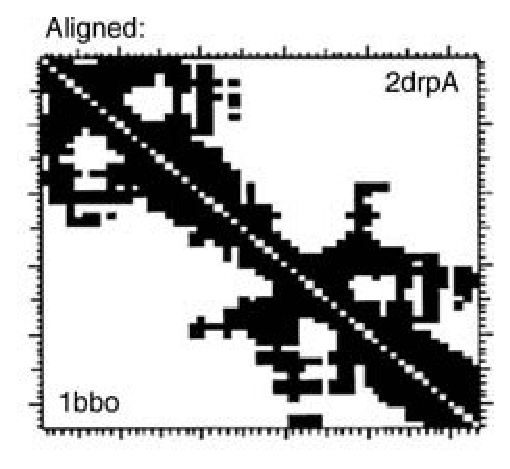
\includegraphics{dali}
%\caption%[]
%{
%Alineamiento DALI de matrices de contactos/distancias, tomado de \cite{Holm2006}. 
%Estas matrices se pueden calcular por ejemplo con RRDistMaps, 
%que es parte de \htmladdnormallink{CHIMERA}{http://rbvi.ucsf.edu/chimera/download.html}.
%}
%\label{fig:dali}
%\end{center}
%\end{figure}

\begin{figure}
\begin{center} 
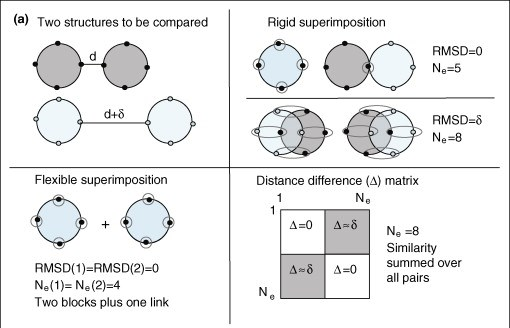
\includegraphics{3Dsuper}
\caption%[]
{
Tres estrategias (r\'{i}gida, flexible y el\'{a}stica) para comparar la estructura terciaria de dos prote\'{i}nas 
con dos dominios (c\'{i}rculos) con 4 residuos cada uno, separados por una secuencia de longitud variable.
Arriba derecha: la superposici\'{o}n r\'{i}gida tiene dos opciones: alinear un total de 5 residuos equivalentes ($Ne$) con RMSD bajo 
o alinear todos ($Ne=8$) con un RMSD alto. 
Abajo izquierda: una superposici\'{o}n flexible rompe la estructura larga en dos subestucturas para optimizar el RMSD sobre 4 residuos en cada dominio.
Abajo derecha: la comparaci\'{o}n de matrices de distancias permite alinear ambos dominios maximizando $Ne$.
Figura tomada de \citet{Hasegawa2009} y reproducida con permiso.
}
\label{fig:dali}
\end{center}
\end{figure}


\begin{figure}
\begin{center} 
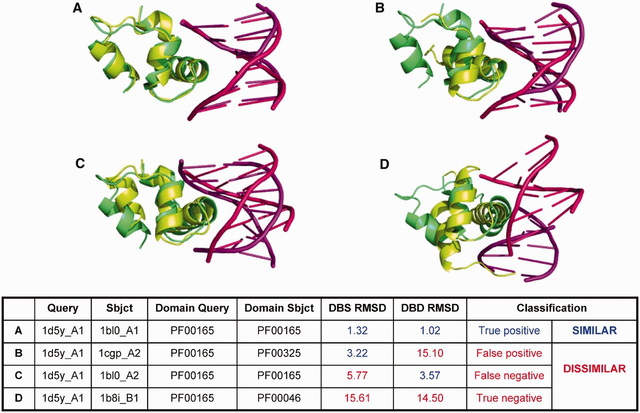
\includegraphics{tfcompare}
\caption%[]
{
Superposiciones de dominios de uni\'{o}n a DNA (DBD) de factores de transcripci\'{o}n, que ponen de manifiesto 
su mecanismo, no siempre conservado, de reconocimiento de sus cis-elementos (DBS). 
Figura tomada de \citet{Sebastian2013}.
}
\label{fig:tfcompare}
\end{center}
\end{figure}

Hay disponibles muchos otros programas disponibles para la comparaci\'{o}n estructural de prote\'{i}nas, 
y cada usuario tiene el suyo preferido. A qu\'{e} se debe esto? 
La raz\'{o}n es que no existe una definici\'{o}n totalmente satisfactoria del alineamiento estructural correcto, 
que es en definitiva la funci\'{o}n que todos estos algoritmos tratan de optimizar. De hecho, ni siquiera
est\'{a} claro si las taxonom\'{i}as estructurales cl\'{a}sicas, 
como \htmladdnormallink{CATH}{http://www.cathdb.info} o
\htmladdnormallink{SCOP}{http://scop.berkeley.edu} \citep{Csaba2009},
son compatibles con la evidencia disponible sobre la evoluci\'{o}n de los plegamientos (\italics{folds}), que
actualmente se imagina como un proceso discreto s\'{o}lo hasta cierto punto \citep{Taylor2002,Pascual2009,Sadowski2010,Andreeva2014}. 
De hecho \htmladdnormallink{SCOP2}{http://scop2.mrc-lmb.cam.ac.uk/} se hizo para superar esas limitaciones.
Otra complicaci\'{o}n adicional es que algunos plegamientos pueden verse como permutaciones circulares de elementos de estructura 
secundaria de otros \citep{Schmidt-Goenner2010}.

A pesar de estas dificultades, en general aceptamos que cada superfamilia de prote\'{i}nas es un \textbf{cl\'{u}ster}
de estructuras muy similares, que se pueden superponer aunque su secuencia sea muy diferente, 
y que cada plegamiento es un subconjunto de superfamilias que comparten una topolog\'{i}a de estructura secundaria.

Lo habitual cuando se publica un nuevo m\'{e}todo es compararlo con otros preexistentes. Estas comparaciones, 
si son rigurosas y reproducibles, pueden ayudar en la tarea de seleccionar un programa id\'{o}neo 
para esta tarea. El algoritmo MAMMOTH, con el que vamos a trabajar, se resume en estos pasos, 
en palabras textuales de sus autores \citep{Ortiz2002}:
\begin{quote}
 1.- From the Calpha trace,  compute the unit-vector  U-RMS  between
 all pairs of heptapeptides of both model and experimental structure.
 The  U-RMS is  described  in:  Kedem, Chew & Elber  (1999)  Proteins
 37(4):554-64,  and  in  Chew, Huttenlocher, Kedem & Kleinberg (1999)
 J.Comp.Biol. 6, 313-325.  This is a measure sensitive  to  the local
 structure.

  2.- Use the matrix derived in step 1 to find and alignment of local
 structures that maximizes the local similarity of both the model and
 the  experimental structure. For that, use a global alignment method 
 with  zero  end  gaps,  as  described  in  Needleman & Wunsch (1970) 
 J.Mol.Biol. 48, 443-453.

  3.- Find the maximum subset of similar  local  structures that have
 their corresponding  Calphas  close  in  cartesian space. "Close" is
 considered here  as  a distance less or equal than 4.0 A. The method
 to  find this subset is a small variant of the MaxSub algorithm from
 the  Fischer  group:  Siew,  Elofsson,  Rychlewski  & Fischer (2000)
 Bioinformatics, in press.

  4.- Obtain  the  probability  of  obtaining the given proportion of
 aligned residues (with respect to the  shortest  protein  model)  by
 chance.  This  metric  (E-value) is then used as the final score (or 
 the  corresponding Z-score, both are equivalent for gaussian distri-
 butions, however the Z-score is a more manegable index). In order to
 obtain this  value, an approach similar to that of Levitt & Gerstein 
 (1998) PNAS 95, 5913 is used, as  described  in  Abagyan  &  Batalov 
 (1997) J.Mol.Biol. 273, 355-368.  The E-value estimation is based on
 extreme-value fitting.  In  a  test  set  with the SCOP database, it 
 shows rather good performance.
\end{quote}
 
MAMMOTH fue comparado con varios m\'{e}todos, como se ve en esta figura:  

\begin{figure}
%\htmlimage{scale=0.5}
\begin{center} 
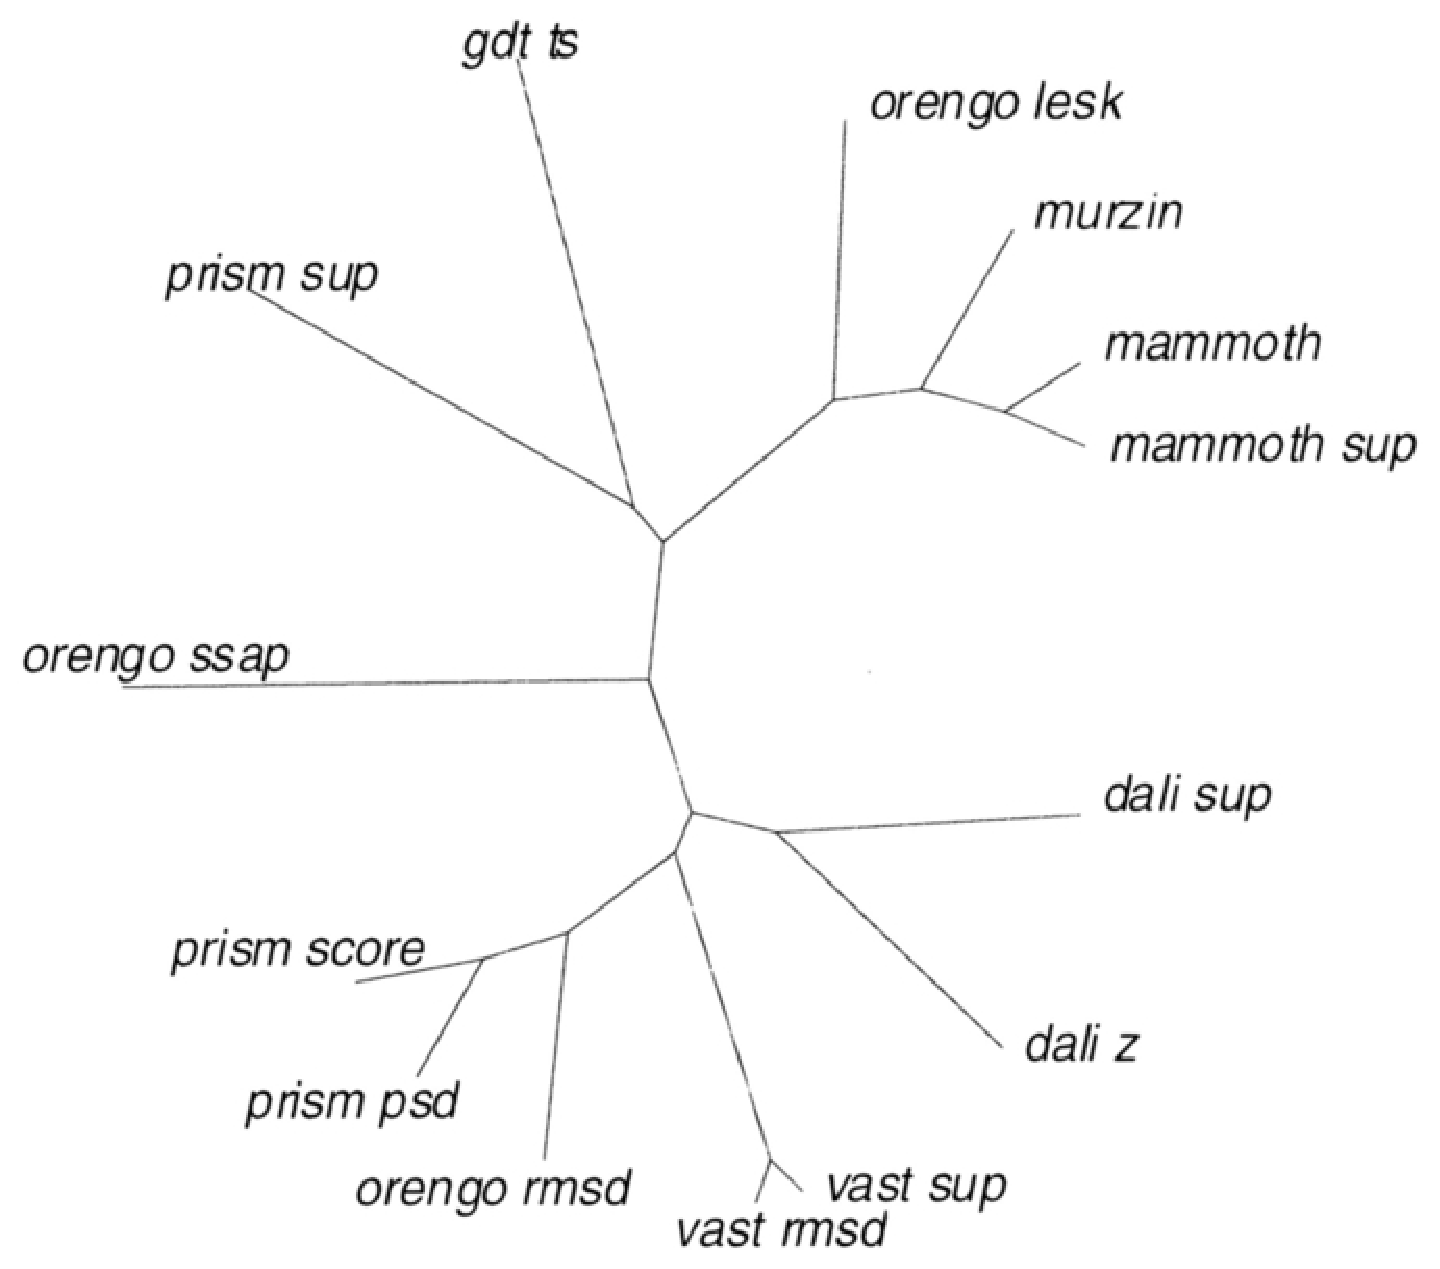
\includegraphics{mammoth_bench}
\caption%[]
{
Semejanza de MAMMOTH respecto a otros algoritmos de comparaci\'{o}n de estructura de prote\'{i}nas, 
incluyendo el criterio de un experto humano (Murzin). Figura tomada de \citet{Ortiz2002}. Copyright (2002) Protein Science.
}
\label{fig:mammoth}
\end{center}
\end{figure}
%$https://www.ncbi.nlm.nih.gov/pmc/articles/PMC2373724/

MAMMOTH es junto con DALI de los mejores programas, porque adem\'{a}s de generar superposiciones y alineamientos satisfactorios, 
sus medidas num\'{e}ricas de similitud devuelven valores que se ajustan a la evaluaci\'{o}n visual de la superposici\'{o}n obtenida.
En concreto, MAMMOTH devuelve para cada alineamiento una puntuaci\'{o}n y su valor esperado asociado (\italics{E-value}),
que podemos interpretar de manera an\'{a}loga a los valores esperados de BLAST, superando las limitaciones del RMSD para 
comparar estructuras que solamente se parecen en algunas regiones \citep{Siew2000}. 
Adem\'{a}s, hay una versi\'{o}n de MAMMOTH que permite calcular 
\htmladdnormallink{alineamientos m\'{u}ltiples}{https://ub.cbm.uam.es/software/mammothm.php}.

Para superar las limitaciones del RMSD, que da el mismo peso a regiones del core que a regiones divergentes, 
\citet{Zhang2004} propusieron otra funci\'{o}n, el TM-score, que disminuye el peso de las parejas alineadas a mayor distancia, es menos sensible
a la longitud de las estructuras comparadas y toma valores entre 0 y 1: 

\begin{equation}
TMscore = max[  \frac{1}{L_{Q}}  \sum_{i=1}^{L_{T}} \frac{1}{ 1 + (\frac{d_{i}}{d_{0}})^{2} } ]
\end{equation} 

Aqu\'{i} $max$ es el valor m\'{a}ximo obtenido en todas las superposiciones calculadas, 
$L_{Q}$ es la longitud de la estructura Q o \italics{query}, 
$L_{T}$ es el total de residuos alineados a la estructura T o \italics{template}, 
$d_{i}$ es la distancia entre la pareja $i$ de residuos y 
$d_{0}$ el factor de escala para normalizar por longitud de secuencia. 

Para calcularlo de manera \'{o}ptima podemos usar su algoritmo TM-align \citep{Zhang2005}, cuyo c\'{o}digo fuente esta disponible en 
\htmladdnormallink{TMalignc.tar.gz}{http://zhanglab.ccmb.med.umich.edu/TM-align/TM-align-C/TMalignc.tar.gz}. La funci\'{o}n TM-score
se ha convertido en el est\'{a}ndar para medir el parecido entre estructuras, ya que se acepta que un valor de 0.5 garantiza un plegamiento similar.

De todos modos, hay una gran variedad de software para esta tarea, 
como se muestra por ejemplo en esta \htmladdnormallink{lista de la WikipediA}{http://en.wikipedia.org/wiki/Structural_alignment_software}.

%\subsection{Ejercicios de similitud estructural entre estructuras proteicas con MAMMOTH}
Para aprender a hacer alineamientos/superposiciones estructurales, y a interpretarlos, podemos hacer este ejercicio:

\begin{itemize}

\item Visita \htmladdnormallink{SCOPe}{http://scop.berkeley.edu}, 
elige una clase (ver figura \ref{fig:foldclassif})
%elige la opci\'{o}n \italics{Enter SCOP at the top of the hierarchy} 
y selecciona un grupo de 5 estructuras de prote\'\i{}nas que pertenezcan a la misma superfamilia, para despu\'{e}s
\begin{itemize}
\item descargar los archivos PDB correspondientes,que contienen las coordenadas at\'{o}micas,  del
\htmladdnormallink{Protein Data Bank}{http://www.rcsb.org/pdb} y
\item compara al menos una pareja de estructuras con MAMMOTH %\htmladdnormallink{MAMMOTH}{https://ub.cbm.uam.es/software/mammoth.php} 
e inspecciona los archivos de salida generados (\verb+maxsub_sup.pdb,maxsub_sup2.pdb,rasmol.tcl+)
%o con la versi\'{o}n \htmladdnormallink{web}{https://ub.cbm.uam.es/software/online/mammoth.php})
\item (el ejecutable se encuentra en \verb+/home/compu2/algoritmos3D/soft/mammoth-1.0-src+)
\end{itemize}
 
\item Visualiza la superposici\'{o}n generada,  con Rasmol (usando la opci\'{o}n \verb+ -script rasmol.tcl+) y con PyMOL

\item Puedes probar a superponer estructuras directamente en \htmladdnormallink{PyMOL}{https://pymol.org/dokuwiki/doku.php?id=command:align}

\item Prueba MAMMOTH con el fin de comparar una estructura problema (una de las 5) contra una biblioteca
de estructuras en formato PDB (las otras 4), como si fuera BLAST. Cu\'{a}l de las 4 estructuras ser\'{i}a el mejor molde o \italics{template})
Cu\'{a}l es el l\'{i}mite esperado de precisi\'{o}n, en t\'{e}rminos de RMSD, que alcanzar\'{i}amos con cada molde?

\item Calcula para algunas de las superposiciones el \htmladdnormallink{TM-score}{http://zhanglab.ccmb.med.umich.edu/TM-score/}.

%Por ejemplo puedes comparar la luciferasa bacteriana 
%\htmladdnormallink{LuxA}{http://www.rcsb.org/pdb/explore/explore.do?structureId=1LUC} con las entradas de la
%biblioteca que puedes descargar de este \htmladdnormallink{enlace}{./files/scoplibrary.tgz} (3.7Mb).
\end{itemize}
 %comparacion y alineamiento estructural de proteinas (MAMMOTH): explicar e-values
%\section{\italics{Protein fold recognition}} \label{FRsection}

Al analizar secuencias gen\'{o}micas frecuentemente encontraremos marcos de lectura (te\'{o}ricos) que codifican para prote\'{i}nas que aparentemente no se parecen a ninguna otra (llamadas a veces \italics{orphans} en la literatura), 
o que s\'{o}lo tienen similitudes obvias con prote\'{i}nas de funci\'{o}n desconocida. Esto puede deberse a que de veras son 
mol\'{e}culas observadas por primera vez, o como vimos en \ref{3dcons}, a que la evoluci\'{o}n ha conservado en mayor grado
la estructura y topolog\'{i}a de las prote\'{i}nas hom\'{o}logas que sus secuencias. 

La segunda posibilidad ha justificado una familia de m\'{e}todos llamados gen\'{e}ricamente de \italics{Fold Recognition} (FR), 
que tienen como objeto reconocer a qu\'{e} tipo de plegamiento (de los conocidos) se debe asignar una secuencia problema, 
especialmente cuando b\'{u}squedas m\'{a}s convencionales con 
\htmladdnormallink{BLAST}{http://blast.ncbi.nlm.nih.gov/Blast.cgi} o 
\htmladdnormallink{FASTA}{http://www.ebi.ac.uk/Tools/fasta/index.html}
han fracasado.
Hist\'{o}ricamente algunos de estos m\'{e}todos se han llamado de
\htmladdnormallink{\italics{threading}}{http://en.wikipedia.org/wiki/Threading_\%28protein_sequence\%29}, 
ya que ciertos algoritmos 
literalmente enhebran la secuencia problema en patrones de coordenadas conocidas, normalmente un subconjunto no redundante
del PDB, para ver si es compatible con alguno, como en la siguiente figura:

\begin{figure}
\begin{center} 
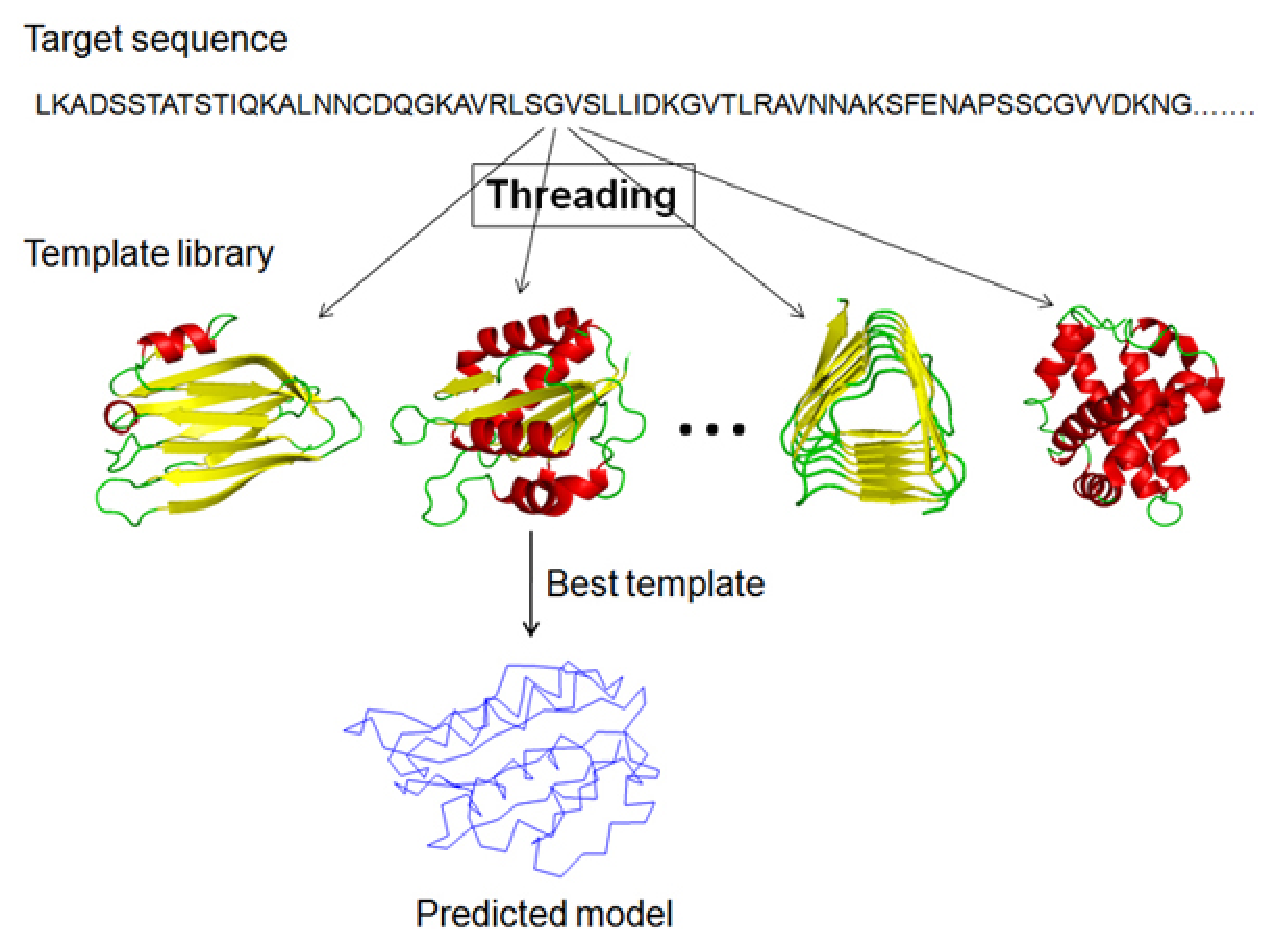
\includegraphics{threading}
\caption%[]
{
Diagrama de flujo de los algoritmos de reconocimiento de plegamiento (FR).
Figura tomada de \cite{Guo2008}. Copyright (2008) Frontiers in Bioscience. 
}
\label{fig:threading}
\end{center}
\end{figure}

El problema de FR lo podemos plantear as\'{i}:
\begin{itemize}
\item \textbf{PROBLEMA:} conocemos la secuencia de una prote\'{i}na, pero desconocemos su tipo de plegamiento y su funci\'{o}n
\item \textbf{SOLUCI\'{O}N PROPUESTA:} comparar la secuencia con todos los plegamientos conocidos, calcular el grado de parecido/compatibilidad con cada uno de ellos y devolver una lista ordenada
\end{itemize}

Se han publicado muchos algoritmos diferentes de FR; en todos ellos de alguna manera se asigna una estructura T a una secuencia A:
\begin{itemize}
\item Por medio de b\'{u}squedas PSI-BLAST bidireccionales transitivas \citep{Koretke2002}. 
La idea es que si buscamos secuencias hom\'{o}logas a partir de A llegamos a encontrar, en alguna iteraci\'{o}n, 
la secuencia T entre los resultados con cierta significancia estad\'{i}stica. De la misma manera, a partir de la secuencia de T llegamos a la secuencia A.

%(\htmladdnormallink{Pubmed}{http://www.ncbi.nlm.nih.gov/pubmed/12021456})
\item Representando cada plegamiento o \italics{fold} por medio de las secuencias conocidas que se pliegan en esa conformaci\'{o}n
y comparten estructura secundaria. Esto se puede hacer por medio de perfiles de secuencia \citep{Gribskov1987}, 
que son matrices sustituci\'{o}n de amino\'{a}cidos espec\'{i}ficas de posici\'{o}n, 
%\htmladdnormallink{perfiles}{http://www.ncbi.nlm.nih.gov/pubmed/3474607} 
o \htmladdnormallink{modelos ocultos de Markov}{http://en.wikipedia.org/wiki/Hidden_Markov_model}, 
que modelan expl\'{i}citamente con qu\'{e} probabilidad se pueden emitir secuencias compatibles con ese plegamiento.

\item Por medio de alineamientos secuencia-perfil %\htmladdnormallink{secuencia-perfil}{http://www.ncbi.nlm.nih.gov/pubmed/12169530} 
o los m\'{a}s sensibles perfil-perfil \citep{Soding2005} %\htmladdnormallink{perfil-perfil}{http://www.ncbi.nlm.nih.gov/pubmed/15531603}, 
que son la raz\'{o}n del \'{e}xito del servidor \htmladdnormallink{HHpred}{https://toolkit.tuebingen.mpg.de/#/tools/hhpred}.

\item Usando potenciales estad\'{i}sticos para evaluar la cercan\'{i}a de los residuos de una secuencia
dado un plegamiento (lo que llamamos \italics{threading} \citep{Threader1992}). Estos m\'{e}todos requieren precalcular,
sobre una colecci\'{o}n de plegamientos no redundantes, con qu\'{e} frecuencia y a qu\'{e} distancia se forman 
parejas de residuos en las estructuras conocidas. %(\htmladdnormallink{genTHREADER}{http://www.ncbi.nlm.nih.gov/pubmed/10191147})

%\item ombinando diferentes moldes, alineamientos y algoritmos en estrategias de b\'{u}squeda de consenso, 
%con la ayuda de m\'{e}tricas fiables como \htmladdnormallink{3D-Jury}{http://www.ncbi.nlm.nih.gov/pmc/articles/PMC2040163/} \citep{Ginalski2003}

%\item Partiendo la secuencia problema en fragmentos, como una estrategia divide y vencer\'{a}s, buscando la estructura
%mas probable para cada fragmento por \italics{threading} \citep{Wu2010}

\end{itemize}

Probablemente la mejor manera de evaluar objetivamente y elegir un m\'{e}todo de FR 
son experimentos colectivos a ciegas con secuencias cuyas estructuras experimentales se hacen p\'{u}blicas
tras las entrega de las predicciones. Hay dos tipos de experimentos de estipo: 
\htmladdnormallink{CASP}{http://predictioncenter.org/index.cgi?page=public_serv}, 
que mide bianualmente la competencia de los algoritmos de los grupos participantes, y 
\htmladdnormallink{CAMEO}{https://www.cameo3d.org}, que hace evaluaciones continuas no supervisadas.

En palabras de \citet{Kelley2015}, desarrollador principal de 
\htmladdnormallink{Phyre2}{http://www.sbg.bio.ic.ac.uk/phyre2}, uno de los m\'{a}s completos,
los mejores predictores tienen resultados indistinguibles en la mayor parte de los casos,
pero en los casos mas complejos desde hace tiempo destaca por su consistencia y 
superiores resultados \htmladdnormallink{I-TASSER}{http://zhanglab.ccmb.med.umich.edu/I-TASSER}.

%En la pr\'{a}ctica, a menudo los usuarios recurrimos a
%\htmladdnormallink{metaservidores}{http://en.wikipedia.org/wiki/Metaserver} como
%\htmladdnormallink{BioInfobank}{http://meta.bioinfo.pl}, desde donde podemos mandar una secuencia problema 
%a muchos servidores de FR, y lo que es m\'{a}s importante, donde podemos evaluar de una manera fiable 
%la calidad de los resultados usando m\'{e}tricas basadas en consensos, como 
%%\htmladdnormallink{2003}{http://bioinformatics.oxfordjournals.org/cgi/reprint/19/8/1015} y 
%\htmladdnormallink{3D-Jury}{http://www.ncbi.nlm.nih.gov/pmc/articles/PMC2040163/} \citep{Ginalski2003}, 
%como podemos comprobar inspeccionando la \htmladdnormallink{tabla de resultados}{http://meta.bioinfo.pl/queue.pl} de BioInfobank.

Estas herramientas web son adecuadas para estudiar unas pocas secuencias, pero si queremos hacer un experimento de FR 
a gran escala, entonces buena idea instalar localmente el software elegido, como por ejemplo
\htmladdnormallink{hh-suite}{https://github.com/soedinglab/hh-suite}, el software que da vida a 
\htmladdnormallink{HHpred}{https://toolkit.tuebingen.mpg.de/#/tools/hhpred}.

El siguiente programa es un prototipo de alineamiento perfil-perfil que usa adem\'{a}s predicciones de estructura secundaria (ver figura \ref{fig:psipred}) 
para guiar el alineamiento. Es un algoritmo de programaci\'{o}n din\'{a}mica, que puedes comprender mejor con ayuda 
del \htmladdnormallink{\italics{Sequence Alignment Teacher}}{http://protein.bio.puc.cl/websoftware/web/?sid=3} \citep{Ibarra2010}.

Para probarlo necesitaras descargar los archivos de entrada
(\htmladdnormallink{1ngk\_A.pssm}{./files/1ngk_A.pssm},\htmladdnormallink{1s69\_A.pssm}{./files/1s69_A.pssm},
\htmladdnormallink{1ngk\_A.psipred}{./files/1ngk_A.psipred},\htmladdnormallink{1s69\_A.psipred}{./files/1s69_A.psipred}):
\verbatiminput{code/prog3.2.pl}
 %fold recognition/threading hhpred
%\section{Modelado de prote\'\i{}nas por homolog\'{i}a} \label{CM}

Con las herramientas que hemos estado manejando ya estamos preparados para modelar prote\'\i{}nas. 
En este contexto modelar significa hacer una predicci\'{o}n de c\'{o}mo se disponen los \'{a}tomos 
de una prote\'\i{}na conocida su secuencia, con el fin de estudiar su funci\'{o}n molecular, su historia evolutiva o, 
si el modelo es bueno, dise\~nar o muestrear ligandos e incluso calcular sus afinidades \citep{Singh2010}. 
Asimismo este tipo de modelos se usan mucho para estudiar el efecto de mutaciones puntuales \citep{Kellogg2011}.

\begin{itemize}
\item \textbf{PROBLEMA:} disponemos de la secuencia de una prote\'{i}na A y quisi\'{e}ramos conocer, aunque sea de manera aproximada, 
su estructura tridimensional
\item \textbf{SOLUCI\'{O}N PROPUESTA:} estimar coordenadas cartesianas para la mayor\'{i}a de los \'{a}tomos de A, 
en base a la estructura conocida de prote\'{i}nas  similares, que llamamos plantillas, moldes, o \italics{templates}
\end{itemize}

Esta metodolog\'{i}a se llama modelado comparativo o por homolog\'{i}a y se describe en profundidad en este
art\'\i{}culo de \citet{Fiser2003}. %\htmladdnormallink{art\'\i{}culo}{./papers/modeller2003.pdf} 
Hay fundamentalmente dos estrategias, que en general requieren alineamientos entre la secuencia problema y los posibles moldes:
\begin{itemize}

\item Ensamblaje de grandes fragmentos r\'{i}gidos, incluso el plegamiento entero, 
obtenidos de estructuras similares alineadas por medio de su secuencia primaria y secundaria
(\htmladdnormallink{SWISS-MODEL}{http://swissmodel.expasy.org}, 
\htmladdnormallink{IntFOLD}{http://www.reading.ac.uk/bioinf/IntFOLD}, 
\htmladdnormallink{ROBETTA}{http://robetta.bakerlab.org} o 
%\htmladdnormallink{3D-JIGSAW}{http://bmm.cancerresearchuk.org/~3djigsaw} 
\htmladdnormallink{MEDELLER}{http://opig.stats.ox.ac.uk/webapps/medeller/home.pl?app=MEDELLER} para prote\'{i}nas transmembrana).
Esta metodolog\'{i}a corta y pega literalmente fragmentos del esqueleto pept\'{i}dico de estructuras conocidas.

\item Modelado por satisfacci\'{o}n de restricciones (distancias, \'{a}ngulos) moleculares extra\'{i}das 
de bases de datos y estructuras similares alineadas (\htmladdnormallink{MODELLER}{https://salilab.org/modeller/}). 
Este m\'{e}todo, conceptualmente similar a la resoluci\'{o}n por NMR (ver secci\'{o}n \ref{metodosExp}), 
produce un conjunto de estructuras para la secuencia A, 
todas ellas compatibles con las restricciones observadas en los \italics{templates}.

\end{itemize}

El algoritmo gen\'{e}rico de modelado comparativo puede dividirse en varios pasos, ilustrados en la figura \ref{fig:CMflow}:
\begin{itemize}
\item{1.} Identificar por similitud de secuencia dominios $D_{1..d}$ en la prote\'\i{}na $S$ que queremos modelar.
\item{2.} Buscar y alinear estructuras molde $M_{1..m}$ que nos sirvan para modelar uno o m\'{a}s dominios de $S$. 
Cada dominio con al menos un molde es potencialmente modelable.
\item{3.} Para cada dominio $D_{i}$ modelable:
\begin{itemize}
\item{3.1.} Refinar el alineamiento local de cada segmento alineado del molde.
\item{3.2.} Tomar las coordenadas pept\'{i}dicas (o descriptores moleculares) de la estructura molde alineada.
\item{3.3.} Copiar los \htmladdnormallink{rot\'{a}meros}{http://kinemage.biochem.duke.edu/databases/rotamer.php}
de las cadenas laterales de los amino\'{a}cidos conservados en el alineamiento.
\item{3.4.} Modelar los rot\'{a}meros de los residuos que mutan respecto al molde, 
con ayuda de una \htmladdnormallink{biblioteca}{http://dunbrack.fccc.edu/bbdep2010}.
\begin{figure}
\begin{center} 
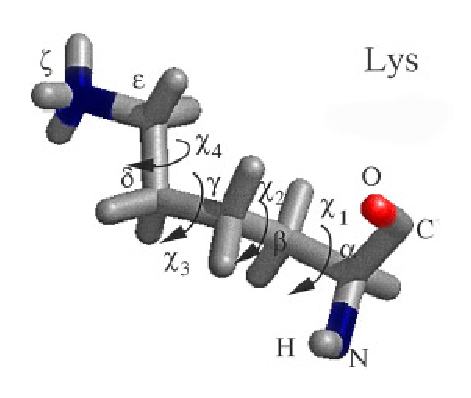
\includegraphics{rotamer}
\caption%[]
{
\'{A}ngulos que definen los rot\'{a}meros de las cadenas laterales.
%figura tomada de \htmladdnormallink{http://bopwww.biologie.uni-freiburg.de}{http://bopwww.biologie.uni-freiburg.de/students/labs/synopsis_jul02/index.html}.
}
\label{fig:rotamer}
\end{center}
\end{figure}
\item{3.4.} A\~nadir los segmentos, normalmente \htmladdnormallink{\italics{loops}}{http://bmm.cancerresearchuk.org/loop}, 
correspondientes a \italics{gaps} en la secuencia alineada del molde.
\item{3.5.} Refinar 1 \'{o} m\'{a}s modelos completos $P_{n}$ con el objeto de eliminar errores obvios de estructura, como impedimentos o choques est\'{e}ricos.
\item{3.6.} Evaluar los modelos $P_{n}$  y estimar su calidad, por medio de aplicaciones como 
\htmladdnormallink{ProQ3}{http://proq3.bioinfo.se},
\htmladdnormallink{Verify3D}{http://services.mbi.ucla.edu/Verify_3D} o 
\htmladdnormallink{FiltRest3D}{http://filtrest3d.genesilico.pl/filtrest3d/index.html}.
\end{itemize}
\end{itemize}

El paso 2 es el m\'{a}s determinante sobre la calidad del modelo y de hecho marca el techo de precisi\'{o}n de la metodolog\'{i}a 
\citep{ContrerasMoreira2005}. Es adem\'{a}s un paso cr\'{i}tico en el sentido de que si el alineamiento $M_{i}$ es malo, 
el modelo resultante ser\'{a} malo, como ya vislumbramos en la secci\'{o}n \ref{3dcons}. Para modelos complicados ser\'{a} 
necesario explorar diferentes combinaciones de moldes y alineamientos para encontrar la mejor soluci\'{o}n. %\citep{Contreras-Moreira2003}.
Si la secuencia problema es multidominio o multim\'{e}rica puede ser necesario modelar su estructura cuaternaria \citep{Tramontano2017}, 
con herramientas especiales como
\htmladdnormallink{BAM}{http://dunbrack.fccc.edu/BAM} o 
\htmladdnormallink{AIDA}{http://ffas.burnham.org/AIDA}.

Con el objeto de explicar en mayor detalle el algoritmo, el siguiente c\'{o}digo implementa los pasos 3.1 y 3.2, quiz\'{a}s
los m\'{a}s fundamentales tras el el paso 2. El programa usa como ejemplo secuencias
y estructuras ya utilizadas en el apartado \ref{3dcons} (\htmladdnormallink{1gd6.pdb}{./files/1gd6.pdb}):
\verbatiminput{code/prog3.3.py}

Como en otros campos de la biolog\'{i}a computacional, el repertorio de software para modelar prote\'{i}nas es muy extenso,
y constantemente incluye nuevas herramientas que sustituyen a otras que envejecen.
Un buen punto de partida para elegir la mejor soluci\'{o}n son los \italics{rankings} que actualiza cada dos a\~nos 
\htmladdnormallink{CASP}{http://predictioncenter.org/index.cgi?page=public_serv}, aunque probablemente los 
programas de modelado preferidos por los usuarios son SWISS-MODEL en la Web y MODELLER como instalable.

\begin{figure}
%\htmlimage{scale=0.5}
\begin{center} 
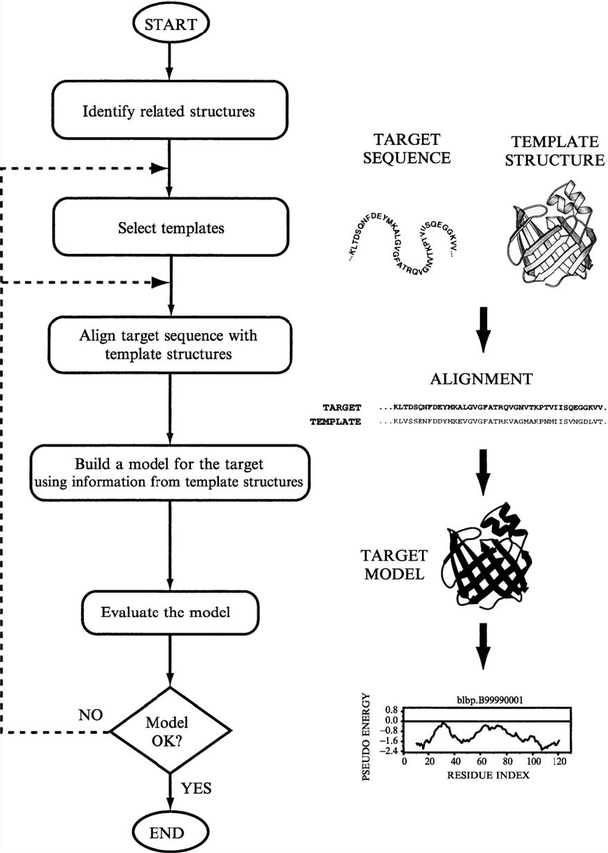
\includegraphics{CMflow}
\caption%[]
{
Algoritmo gen\'{e}rico de modelado comparativo.
Figura tomada de \citet{Fiser2003}. Copyright (2003) Methods in Enzymology.
}
\label{fig:CMflow}
\end{center}
\end{figure}

\begin{figure}
\begin{center} 

\includegraphics{figure_3_contrera_review_final}
\caption%[]
{
Los errores en modelado comparativo se disparan al usar estructuras molde con identidades bajas.
Este comportamiento se observa con diferentes herramientas de modelado, incluyendo SWISS-MODEL.
Figura de \citet{Contreras-Moreira2002b}. 
}
\label{fig:CMbench}
\end{center}
\end{figure}

En la pr\'{a}ctica podemos hacer nuestros modelos por homolog\'{i}a, con la opci\'{o}n de controlar todos los pasos
del procedimiento, por medio del programa \htmladdnormallink{MODELLER}{https://salilab.org/modeller} \citep{Sali1993}, 
disponible sin costo para usuarios acad\'{e}micos. %\verb+/home/bioinfo/bin/modeller8v1/bin/mod8v1+ 
El programa tiene \htmladdnormallink{m\'{u}ltiples posibilidades}{https://salilab.org/modeller/tutorial/}, pero en este ejemplo
nos centramos en el caso m\'{a}s sencillo consistente en hacer un modelo a partir de un s\'{o}lo molde o \italics{template},
estimando su calidad del modelo por medio de la funci\'{o}n DOPE \citep{Shen2006}:
\begin{itemize}

\item Secuencia problema: \htmladdnormallink{FNR}{http://www.expasy.org/uniprot/FNR_ECOLI}, 
regulador transcripcional de \italics{Escherichia coli}.

\item Busca, por ejemplo usando PSI-BLAST, secuencias similares (probablemente hom\'{o}logas)
cuya estructura est\'{e} en el PDB (moldes o \italics{templates}).

\item Para cada uno de los \italics{templates} interesantes sigue estos pasos:
\begin{itemize}

	\item descarga el fichero de coordenadas del \htmladdnormallink{PDB}{http://www.rcsb.org/pdb} 
	y extrae la secuencia S contenida en los campos \verb+ATOM+

	\item alinea la secuencia S de las coordenadas con la secuencia problema (FNR, por ejemplo con 
  \htmladdnormallink{clustal-omega}{https://www.ebi.ac.uk/Tools/msa/clustalo} o usando el mismo alineamiento de BLAST) 
	y crea un archivo con extensi\'{o}n 
	\verb+.ali+ con este formato, donde \verb+structureX+ es el molde, \verb+sequence+ es la secuencia problema o \italics{query} 
	y los dem\'{a}s campos definen el rango de residuos alineados del \italics{template}, y su resoluci\'{o}n:

\begin{verbatim}
C; Alineamiento de muestra en formato PIR
>P1;1PDB
structureX:1PDB:1    :A:106  :A:nombre_template:: 1.90: 
AFVVTDNCIKCKYTDCVEVCPVDCFYEGPNFLVIHPDECIDCALCEPECPAQAIFSEDEVPEDMQEFIQLNAELA
EVWPNITEKKDPLPDAEDWDGVKGKLQHLER*
>P1;query
sequence:query:::::::0.00: 0.00
AYVINDSC--IACGACKPECPVNIIQGS--IYAIDADSCIDCGSCASVCPVGAPNPED-----------------
-------------------------------*
\end{verbatim}

	\item genera un gui\'{o}n o \italics{script} para MODELLER como \verb+guion_nombre_template.py+:

\begin{verbatim}
from modeller.automodel import *   

log.verbose()    
env = environ() 

# 1) directorio donde se encuentran los ficheros con coordenadas de moldes/templates, 
# con extension .pdb,.atm,.ent
env.io.atom_files_directory = './templates/'

# 2) prepara el modelado
a = automodel(env,
              alnfile  = 'alineamiento.ali',  # fichero con el alineamiento
              knowns   = '1PDB',              # nombre del template como aparece en alnfile
              sequence = 'query',             # nombre de secuencia problema como aparece en alnfile
	          assess_methods=(assess.DOPE))      

a.starting_model= 1                           # define cuantos modelos diferentes quieres
a.ending_model  = 2                 
				  
# 3) accion! 
a.make()                  
\end{verbatim}

	\item ahora ejecuta MODELLER (por ejemplo poniendo en el terminal: \verb+$ mod9v8 guion_template.py+ y al terminar revisa 
	\verb+guion_nombre_template.log+ para comprobar la evaluaci\'{o}n emp\'{i}rica del modelo o modelos obtenidos

\end{itemize}
\end{itemize}


%%%%%%%%%%%%%%%%%%%%%%%%%%%%%%%%%%%%%%%%%%%%%%%%%%%%%%%%%%%%%%%%%%%%%%%%%%%%%%%
%%%%%%%%%%%%%%%%%%%%%%%%%%%%%%%%%%%%%%%%%%%%%%%%%%%%%%%%%%%%%%%%%%%%%%%%%%%%%%%


\section{Modelado de prote\'\i{}nas \italics{ab initio}} \label{abinitio}

Hablamos de protocolos \italics{ab initio} cuando tratamos de modelar
el plegamiento de un polip\'{e}ptido solamente a partir de su secuencia y de la f\'\i{}sica  \citep{Baker2001}. 
Sin embargo, los m\'{e}todos de este tipo
m\'{a}s exitosos hasta la fecha reconstruyen la estructura terciaria a base de peque\~{n}os fragmentos cortados 
de estructuras conocidas y seleccionados por similitud de secuencia. 

El mejor ejemplo es el algoritmo Rosetta \citep{Simons1997}, implementado en el servidor web 
\htmladdnormallink{ROBETTA}{http://robetta.bakerlab.org}, 
que permite modelar secuencias cortas cuando no hay moldes que alineen con la secuencia problema, 
ni siquiera por \italics{fold recognition} (ver secci\'{o}n \ref{FRsection}). 
Usa fragmentos de 9 amino\'{a}cidos de longitud. En este caso podemos definir el problema tipo de esta manera:

\begin{itemize}
\item \textbf{PROBLEMA:} disponemos de la secuencia de una prote\'{i}na A y quisi\'{e}ramos conocer, aunque esa de manera aproximada, su estructura tridimensional
\item \textbf{SOLUCI\'{O}N PROPUESTA:} combinar fragmentos tomados de estructuras del PDB, generar conformaciones alternativas y seleccionar las mejores
\end{itemize}

\begin{figure}
\begin{center} 
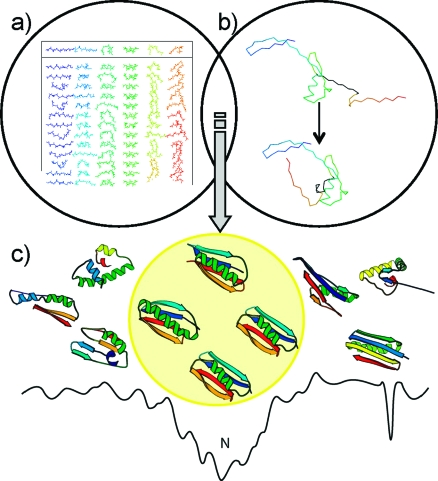
\includegraphics{rosetta}
\caption%[]
{
Resumen del protocolo Rosetta, tomado de \citet{Kaufmann2010}.
A) Se seleccionan de una biblioteca los fragmentos con secuencias mas parecidas a los $K$-meros de la secuencia problema ($K=9$).
B) Combinaci\'{o}n de fragmentos solapantes para generar muchas conformaciones alternativas.
C) Optimizaci\'{o}n de conformaciones con funciones que eval\'{u}an interacciones no locales. 
Copyright (2010) Biochemistry.
}
\label{fig:Rosetta}
\end{center}
\end{figure}

Este tipo de algoritmos requieren tener precalculada una biblioteca de fragmentos de longitud $K$ de estructura conocida,
funciones para seleccionar los mejores fragmentos para cada $K$-mero de la secuencia problema,
funciones de evaluaci\'{o}n que permitan descubrir conformaciones que se parezcan a las nativas, 
y muchos recursos computacionales, dado que todos estos pasos son costosos.
Otro algoritmo que funciona tanto para \italics{fold recognition} como para modelado \italics{ab initio} es 
\htmladdnormallink{I-TASSER}{http://zhanglab.ccmb.med.umich.edu/I-TASSER}:

\begin{figure}
\begin{center} 
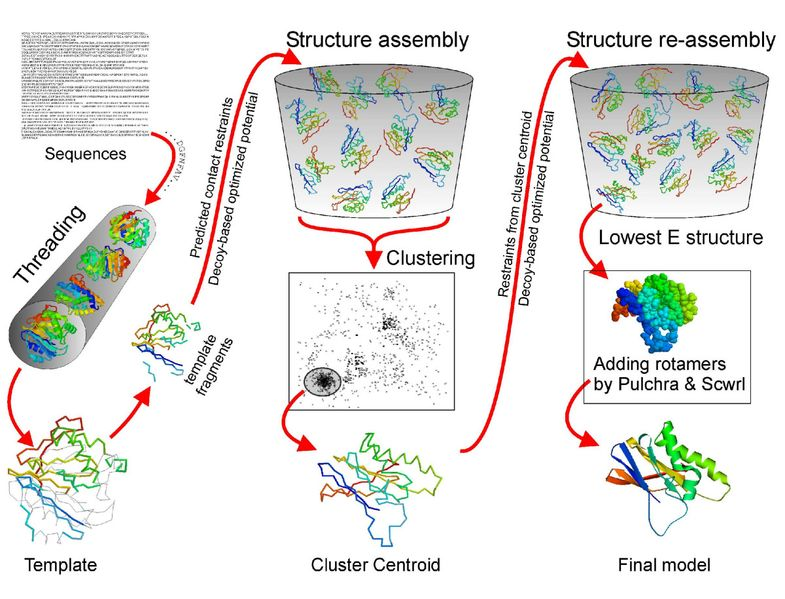
\includegraphics{ITASSER}
\caption%[]
{
Resumen del protocolo TASSER. 
Figura de \citet{Wu2007}, reproducida con permiso de los autores.
}
\label{fig:ITASSER}
\end{center}
\end{figure}
 %modelado comparativo de proteinas (MODELLER): explicar restraints de modeller y rotameros
%\section{Modelado de prote\'{i}nas por predicci\'{o}n de contactos} \label{contactosPred}

Las matrices de contactos (ver secci\'{o}n \ref{estr34})  han sido durante mucho tiempo una fuente de inspiraci\'{o}n de m\'{e}todos 
de predicci\'{o}n estructural, con la idea subyacente de 'si somos capaces de predecir con informaci\'{o}n evolutiva qu\'{e} residuos de 
una secuencia contactan, entonces podremos resolver su estructura' \citep{Gobel1994,deJuan2013}.

La informaci\'{o}n evolutiva en cuesti\'{o}n es normalmente un alineamiento m\'{u}ltiple de secuencias hom\'{o}logas, que se espera
capturen de forma impl\'{i}cita las limitaciones que impone la estructura terciaria de un dominio a las sustituciones de amino\'{a}cidos
que contactan. La funci\'{o}n matem\'{a}tica que se emplea habitualmente para estudiar esto es la 
\htmladdnormallink{informaci\'{o}n mutua}{http://es.wikipedia.org/wiki/Informaci\%C3\%B3n\_mutua} (MI), 
que mide la dependencia entre dos variables, en este caso columnas de un alineamiento.

\begin{figure}
\begin{center} 
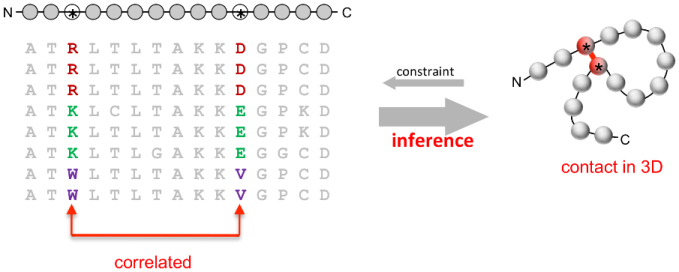
\includegraphics{EVfoldcorr}
\caption%[]
{
Las mutaciones correlacionadas entre columnas de un alineamiento m\'{u}ltiple se pueden emplear para predecir contactos entre residuos en el plegamiento.
Figura tomada de \cite{Marks2011} y reproducida con permiso de los autores.
}
\label{fig:EVfold1}
\end{center}
\end{figure}

Por tanto, el problema de la predicci\'{o}n de contactos se puede plantear as\'{i}:
\begin{itemize}
\item \textbf{PROBLEMA:} conocemos la secuencia de una prote\'{i}na y las de muchas secuencias hom\'{o}logas
\item \textbf{SOLUCI\'{O}N PROPUESTA:} alineamos las secuencias, buscamos posiciones que muestren evidencia de coevoluci\'{o}n 
y buscamos plegamientos compatibles con esos contactos
\end{itemize}

El algoritmo \htmladdnormallink{EVfold}{http://EVfold.org} %, publicado originalmente en \citep{Marks2011}, 
emplea estos elementos
para hacer predicciones de contactos de alta calidad, ya que es capaz de distinguir entre posiciones de la secuencia
que directamente contactan (causativas) de las que correlacionan simplemente porque contactan con un mismo residuo (transitivas). 
Usando su terminolog\'{i}a,
MI es un modelo local de probabilidad de contactos, que ellos son capaces de corregir y convertir en un modelo global usando conceptos 
de la mec\'{a}nica estad\'{i}stica y la maximizaci\'{o}n de la entrop\'{i}a. El modelo global se llama de Informaci\'{o}n Directa (DI)
\citep{Marks2011}.

\begin{figure}
\begin{center} 
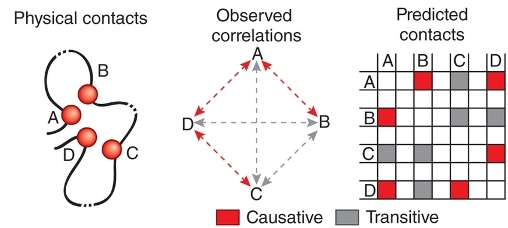
\includegraphics{EVfold22}
\caption%[]
{
Definici\'{o}n de contactos entre residuos (A,B,C,D) y de correlaciones directas y transitivas.
Figura tomada de \cite{Marks2012}. Copyright (2012) Nature Biotechnology.
}
\label{fig:EVfold1.1}
\end{center}
\end{figure} %https://www.ncbi.nlm.nih.gov/pmc/articles/PMC4319528/figure/F2/

\begin{figure}
\begin{center} 
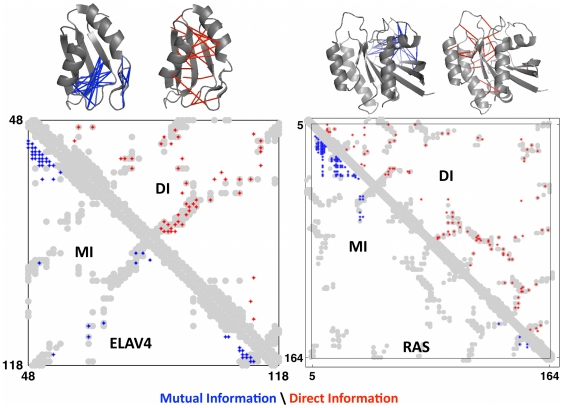
\includegraphics{EVfold3}
\caption%[]
{
La inferencia de contactos entre residuos es mejor con el modelo global (DI, ver texto) que con el modelo local MI.
La figura muestra predicciones de contactos para las prote\'{i}nas ELAV4 (derecha) y RAS (izquierda).
Las predicciones globales se reparten uniformemente por la secuencia y se solapan mejor con los contactos observados en estructuras experimentales.
Figura tomada de \cite{Marks2011} y reproducida con permiso de los autores.
}
\label{fig:EVfold2}
\end{center}
\end{figure}

La siguiente figura muestra el diagrama de flujo completo del m\'{e}todo \htmladdnormallink{EVfold}{http://EVfold.org}, 
que ha sido posteriormente adaptado para prote\'{i}nas transmembrana \citep{Hopf2012} y 
tambi\'{e}n para complejos cuaternarios \citep{Hopf2014}:

\begin{figure}
\begin{center} 
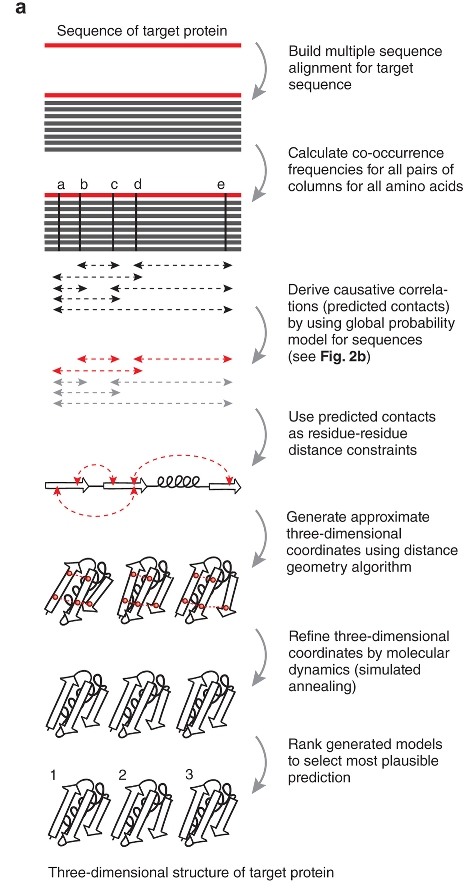
\includegraphics{EVfold21}
\caption%[]
{
Algoritmo de plegamiento de prote\'{i}nas en base a observaciones de mutaciones correlacionadas,
que se transforman en predicciones de contactos, tomado de \cite{Marks2012}. Copyright (2012) Nature Biotechnology.
}
\label{fig:EVfold3} %https://www.ncbi.nlm.nih.gov/pmc/articles/PMC4319528/figure/F2/
\end{center}
\end{figure}

La siguiente figura muestra los resultados de un experimento de validaci\'{o}n de EVfold:

\begin{figure}
\begin{center} 
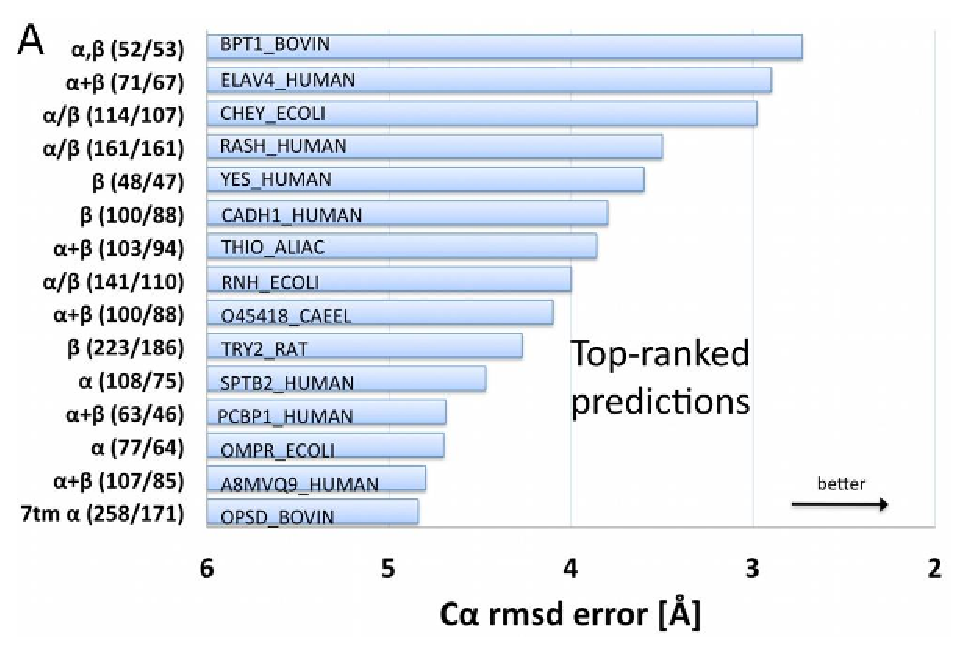
\includegraphics{EVfoldbenchA}
\caption%[]
{
Calidad de las mejores predicciones de EVfold en un conjunto de 15 prote\'{i}nas con diferentes composiciones de estructuras secundaria.
Entre par\'{e}ntesis se muestran el n\'{u}mero de residuos del dominio modelado y 
el n\'{u}mero de residuos sobre los que se calcul\'{o} el RMSD entre el modelo y la estructura experimental.
Figura tomada de \cite{Marks2011} y reproducida con permiso de los autores.
}
\label{fig:EVfold4}
\end{center}
\end{figure}

Esta familia de m\'{e}todos  se est\'{a} desarrollando todav\'{i}a y sigue habiendo avances importantes \citep{Buchan2017}.
El m\'{a}s notable es que el uso de secuencias metagen\'{o}micas permite ampliar el universo de secuencias lo suficiente 
para mejorar las predicciones de contactos (usando por ejemplo \htmladdnormallink{GREMLIN}{http://gremlin.bakerlab.org/submit.php}) 
y obtener as\'{i} estructuras, de momento bacterianas, de numerosos plegamientos desconocidos \citep{Ovchinnikov2017}. 
Adem\'{a}s, \citet{Ovchinnikov2017} proponen una funci\'{o}n para estimar la calidad de los modelos si hay suficientes secuencias para abordar
este tipo de modelado:

\begin{equation}
N_{f} = \frac{clusters_{nr80}}{\sqrt L} 
\end{equation} 

En esta funci\'{o}n el numerador representa el total de clusters de secuencias hom\'{o}logas no redundantes al 80\% 
encontradas con \htmladdnormallink{HHblits}{https://toolkit.tuebingen.mpg.de/#/tools/hhblits} y el numerador es la longitud de la secuencia problema. 
Cuando $N_{f} > 64$ se obtienen modelos de buena calidad. 
 
Para poner en pr\'{a}ctica estos algoritmos se puede realizar el siguiente ejercicio:

\begin{itemize}

\item Visita \htmladdnormallink{UniProt}{http://www.uniprot.org/}, elige una prote\'{i}na y extrae su secuencia S.

\item Busca secuencias similares a S y gu\'{a}rdalas en un archivo.

\item Calcula un alineamiento m\'{u}ltiple A que incluya a S con sus hom\'{o}logos, elimina las secuencias muy cortas y 
guarda el resultado en un fichero FASTA.

\item Con ayuda de los 
\htmladdnormallink{m\'{e}todos suplementarios}{https://doi.org/10.1371/journal.pone.0028766.s017} de \cite{Marks2011}
modifica el c\'{o}digo fuente del programa 3.4 para calcular el peso de las secuencias en base a su identidad
y sumar pseudoconteos y de esa manera calcular con mayor precisi\'{o}n MI en tu alineamiento A.
Hay tambi\'{e}n c\'{o}digo fuente disponible en 
\htmladdnormallink{http://evfold.org/evfold-web/code.do}{http://evfold.org/evfold-web/code.do}.

\item Construye un modelo 3D para S.

\item Edita el archivo PDB del modelo y marca algunas parejas de residuos con valores altos de MI. Para ello puedes usar la columna del factor B,
dejando a '00.00' el resto de residuos. 

\item Visualiza el modelo editado y discute los resultados obtenidos.

\end{itemize}

\verbatiminput{code/prog3.4.pl}

 %modelado 3D en base a contactos
%\section{Mutaciones puntuales de prote\'{i}nas} \label{pointmut}

Un problema que se presenta con cada vez mayor frecuencia desde que llegaron las tecnolog\'{i}as de 
ultrasecuenciaci\'{o}n es el de estimar el fenotipo molecular de un polimorfismo gen\'{e}tico, 
por ejemplo un SNP que cambia la secuencia de amino\'{a}cidos de una prote\'{i}na al provocar 
una sustituci\'{o}n no sin\'{o}nima (\italics{missense}). 
Esto es necesario porque hay muchos m\'{a}s genotipos que fenotipos observados, y porque cu\'{a}nto m\'{a}s se secuencia se hace
patente que los individuos de una especie son portadores de m\'{u}ltiples mutaciones de diferente naturaleza
\citep{Peterson2013}.

Esto se relaciona con los resultados de \citet{Chothia1986}, presentados en la secci\'{o}n \ref{3dcons}, que 
observaron que los efectos de las mutaciones sobre la estructura (y por tanto la funci\'{o}n) dependen en
parte de d\'{o}nde se produzcan. No tiene el mismo efecto cambiar un amino\'{a}cido enterrado que uno en un
\italics{loop}, o uno que coevoluciona con otro de un lazo vecino. Del mismo modo, una sustituci\'{o}n en el interior
de una h\'{e}lice no se puede comparar con la eliminaci\'{o}n de un residuo catal\'{i}tico \citep{Berrondo2011}
o de otro clave para interaccionar con otras prote\'{i}nas \citep{deJuan2013}. 
El muestreo a gran escala de \citet{Rocklin2017} estudi\'{o} la estabilidad de miles de miniprote\'{i}nas (hasta 50aa) sint\'{e}ticas 
y unas 500 naturales del PDB nos ha proporcionado los mejores datos hasta la fecha. En esencia lo que hacen es medir la estabilidad 
de miles de secuencias de amino\'{a}cidos expres\'{a}ndolas y exponi\'{e}ndolas a proteasas en levadura.
De esa manera estiman el efecto que tienen mutaciones individuales dependiendo de su contexto de estructura secundaria, 
ya sea una alfa-h\'{e}lice, una l\'{a}mina beta o un lazo o loop:

\begin{figure}
\begin{center} 
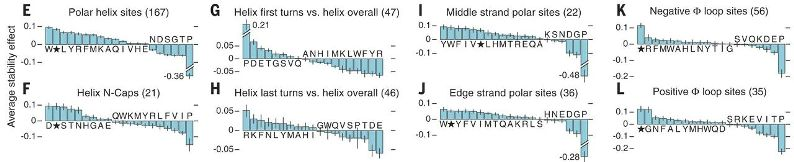
\includegraphics{stabilityTable}
\caption%[]
{
Efecto sobre la estabilidad de mutaciones en diferentes contextos estructurales. 
Los valores negativos, como los de la prolina en general, son desestabilizadores. 
Adaptada de \citet{Rocklin2017}. Copyright (2017) Science.
}
\label{fig:miniprotstab} %https://www.ncbi.nlm.nih.gov/pmc/articles/PMC5568797/
\end{center}
\end{figure}

\begin{figure}
\begin{center} 
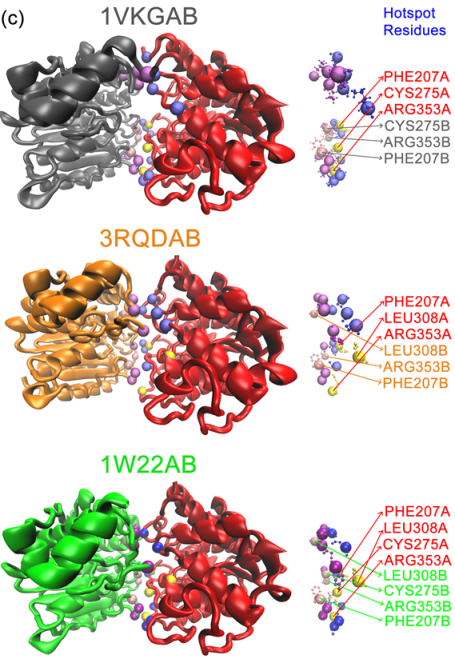
\includegraphics{ppi_interface}
\caption%[]
{
Grafo de la interfaz entre una histona-deacetilasa (en rojo) y tres parejas distintas.
Figura tomada de \citet{Cukuroglu2014} y reproducida con permiso de los autores.
}
\label{fig:ppi_interface}
\end{center}
\end{figure}

%\begin{figure}
%\begin{center} 
%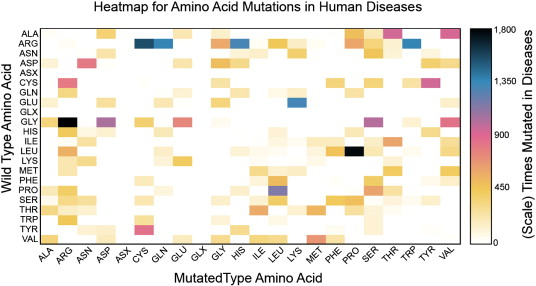
\includegraphics{human_mutations_heatmap}
%\caption%[]
%{
%Frecuencias de sustituci\'{o}n de amino\'{a}cidos en enfermedades humanas.
%Figura tomada de \citet{Peterson2013} y reproducida con permiso.}
%\label{fig:human_mutations_heatmap} %https://www.ncbi.nlm.nih.gov/pmc/articles/PMC3807015/
%\end{center}
%\end{figure}

Como se muestra en la figura \ref{fig:SNPpredictors}, hay una gran variedad de m\'{e}todos para la inferencia del fenotipo
molecular de mutaciones puntuales en prote\'{i}nas, y solamente algunos usan informaci\'{o}n estructural.
Probablemente el m\'{a}s universal de todos sea SIFT \citep{Kumar2009}, que usa como evidencia la
historia evolutiva de cada familia de prote\'{i}nas, que integra entre otras cosas determinantes estructurales
siempre y cuando haya suficientes secuencias hom\'{o}logas conocidas \citep{Saunders2002}. 
Sin embargo, como ocurre a menudo en biolog\'{i}a computacional, no es sencillo averiguar a partir de un
an\'{a}lisis de la literatura qu\'{e} m\'{e}todos son mejores. Hay que probarlos y escoger, y entre los
disponibles haya cada vez m\'{a}s alternativas que hacen un uso expl\'{i}cito de informaci\'{o}n
estructural, en concreto del contexto del residuo sustituido, como PolyPhen-2 \citep{Adzhubei2010},
SusPect \citep{Yates2014} o mCSM \citep{Pires2014}.

\begin{figure}
\begin{center} 
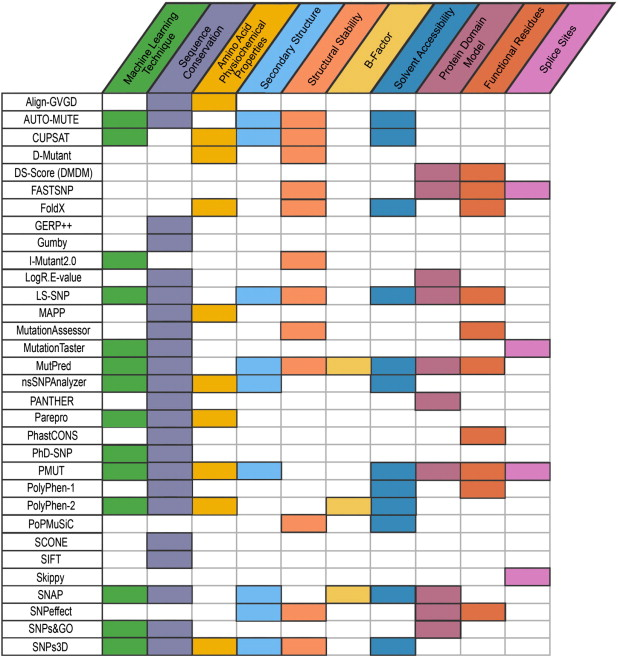
\includegraphics{SNPpredictors}
\caption%[]
{
Clasificaci\'{o}n de m\'{e}todos de inferencia de fenotipos de mutaciones no sin\'{o}nimas en base a los tipos de datos que emplean.
Figura tomada de \citet{Peterson2013} y reproducida con permiso.
}
\label{fig:SNPpredictors}
\end{center}
\end{figure}

\begin{figure}
\begin{center} 
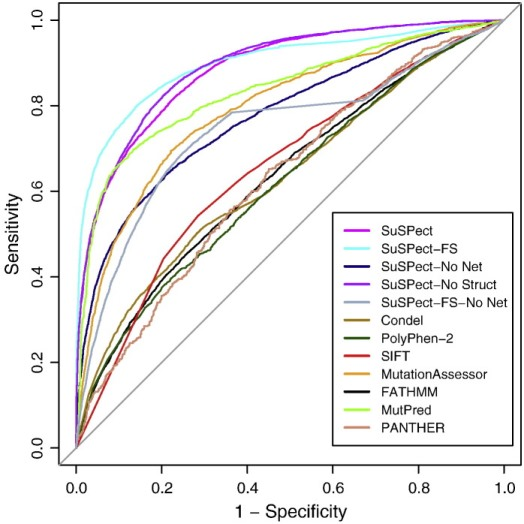
\includegraphics{SNP_performance}
\caption%[]
{
Comparaci\'{o}n del rendimiento de SusPect prediciendo mutaciones humanas delet\'{e}reas frente a otros predictores.
Figura tomada de \citep{Yates2014} y reproducida con permiso.
}
\label{fig:SNP_performance} %https://www.ncbi.nlm.nih.gov/pmc/articles/PMC4087249/
\end{center}
\end{figure}

Para explorar la predicci\'{o}n de fenotipos de mutaciones no sin\'{o}nimas planteo este ejercicio:
\begin{itemize}

\item Visita una base de datos de mutantes, como \htmladdnormallink{OMIM}{http://www.omim.org}, y elige una prote\'{i}na P (ejemplo: OPCML).

\item Obt\'{e}n la secuencia silvestre de amino\'{a}cidos S y al menos otra M con una mutaci\'{o}n delet\'{e}rea.

\item Construye un modelo comparativo de M y S.

\item Haz predicciones de fenotipo para S y M con ayuda, por ejemplo, de: \htmladdnormallink{SIFT}{http://sift.jcvi.org/}, 
\htmladdnormallink{PolyPhen-2}{http://genetics.bwh.harvard.edu/pph2/} y \htmladdnormallink{SusPect}{http://www.sbg.bio.ic.ac.uk/~suspect}.

\item Compara las predicciones obtenidas e interpr\'{e}talas a la luz de las estructuras modeladas. 
Qu\'{e} limitaciones del modelado comparativo afloran?

\end{itemize}
 %prediccion de efecto de mutaciones puntuales

\section{Comparaci\'{o}n de estructura terciaria entre prote\'{i}nas} \label{compS3}

El hecho de que la estructura terciaria est\'{a} m\'{a}s conservada que la secuencia (ver secci\'{o}n \ref{threedeecons})
podemos aprovecharlo para buscar posibles relaciones filogen\'{e}ticas remotas entre prote\'{i}nas:

\begin{itemize}
\item \textbf{PROBLEMA:} disponemos de las coordenadas de dos prote\'{i}nas A y B y queremos calcular cu\'{a}nto se parecen sus estructuras
\item \textbf{SOLUCI\'{O}N:} buscar las subestructuras de m\'{a}ximo tama\~no subA y subB que minimizan la distancia entre \'{a}tomos equivalentes 
(ver secci\'{o}n \ref{threedeecons})
\end{itemize}

Repasemos algunos algoritmos fundamentales para calcular la similitud estructural entre parejas de prote\'{i}nas
(hay alguno m\'{a}s en la \htmladdnormallink{WikipediA}{http://en.wikipedia.org/wiki/Structural_alignment}):
\begin{itemize}

\item Conversi\'{o}n de informaci\'{o}n estructural en secuencias usando un alfabeto a medida para acelerar la comparaci\'{o}n
(\htmladdnormallink{Foldseek}{https://search.foldseek.com/search})

\item Alineamiento estructural iterativo (\htmladdnormallink{STAMP}{http://www.compbio.dundee.ac.uk/downloads/stamp/}). 
El primer borrador de alineamiento se calcula con ayuda de  matrices de sustituci\'{o}n de amino\'{a}cidos como 
\htmladdnormallink{BLOSUM}{https://en.wikipedia.org/wiki/BLOSUM}. \'{E}ste sirve para calcular la superposici\'{o}n correspondiente y 
permite refinar el conjunto de residuos equivalentes, aquellos por debajo de cierto umbral de distancia.
Estas iteraciones de alineamiento y definici\'{o}n de sobconjuntos de residuos equivalentes se repiten hasta que convergen y 
el RMSD no mejora (ver \citet{Chothia1986} y secci\'{o}n \ref{threedeecons}).

\item Doble programaci\'{o}n din\'{a}mica para primero) establecer fragmentos localmente similares entre ambas estructuras y 
segundo) estimar el subconjunto de fragmentos que producen una superposici\'{o}n \'{o}ptima 
(\htmladdnormallink{SSAP}{http://sillitoe.cathdb.info/tools/cath-ssap}). 
M\'{a}s detalles en este \htmladdnormallink{enlace}{http://en.wikipedia.org/wiki/Structural_alignment#SSAP}.

%\item extensi\'{o}n combinatoria de fragmentos alineados localmente (\htmladdnormallink{CE}{http://source.rcsb.org/jfatcatserver/ceHome.jsp})

\item Comparaci\'{o}n de matrices de contactos/distancias (\htmladdnormallink{DALI}{http://ekhidna.biocenter.helsinki.fi/dali_server}).
En vez de trabajar con p\'{e}ptidos en 3D, algo que requiere calcular rotaciones y transforamciones, 
esta familia de m\'{e}todos primero convierten cada estructura a su matriz de distancias correspondiente,
para luego compararlas entre si.

%\item alineamiento iterativo de fragmentos de \italics{backbone} hasta converger en subconjunto equivalente \'{o}ptimo 
%(\htmladdnormallink{MAMMOTH}{http://ub.cbm.uam.es/software/mammoth.php}, \htmladdnormallink{TM-ALIGN}{http://zhanglab.ccmb.med.umich.edu/TM-align})

\item Minimizaci\'{o}n de la informaci\'{o}n requerida para reconstruir las coordenadas de una estructura dadas las de la otra
(\htmladdnormallink{mmligner}{http://lcb.infotech.monash.edu.au/mmligner}). La virtud de este aproximaci\'{o}n es que prescinde 
de la elecci\'{o}n subjetiva de umbrales y define de manera precisa la superposici\'{o}n \'{o}ptima.

\item Superposici\'{o}n de factores de transcripci\'{o}n para deducir el alineamiento correcto de sus sitios \italics{cis} 
(\htmladdnormallink{TFcompare}{https://hub.docker.com/r/eeadcsiccompbio/tfcompare})

\end{itemize}

Puedes ampliar detalles de estos algoritmos en \citet{pascual_garcia_alberto_2014_1066346}.

%\begin{figure}
%\begin{center} 
%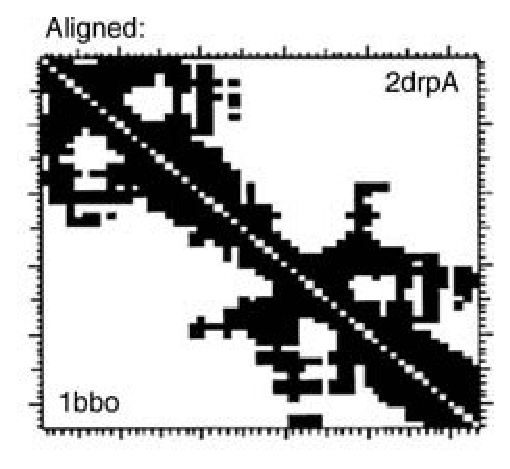
\includegraphics{dali}
%\caption%[]
%{
%Alineamiento DALI de matrices de contactos/distancias, tomado de \cite{Holm2006}. 
%Estas matrices se pueden calcular por ejemplo con RRDistMaps, 
%que es parte de \htmladdnormallink{CHIMERA}{http://rbvi.ucsf.edu/chimera/download.html}.
%}
%\label{fig:dali}
%\end{center}
%\end{figure}

\begin{figure}
\begin{center} 
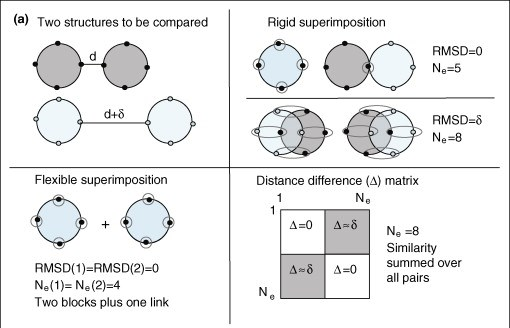
\includegraphics{3Dsuper}
\caption%[]
{
Tres estrategias (r\'{i}gida, flexible y el\'{a}stica) para comparar la estructura terciaria de dos prote\'{i}nas 
con dos dominios (c\'{i}rculos) con 4 residuos cada uno, separados por una secuencia de longitud variable.
Arriba derecha: la superposici\'{o}n r\'{i}gida tiene dos opciones: alinear un total de 5 residuos equivalentes ($Ne$) con RMSD bajo 
o alinear todos ($Ne=8$) con un RMSD alto. 
Abajo izquierda: una superposici\'{o}n flexible rompe la estructura larga en dos subestucturas para optimizar el RMSD sobre 4 residuos en cada dominio.
Abajo derecha: la comparaci\'{o}n de matrices de distancias permite alinear ambos dominios maximizando $Ne$.
Figura tomada de \citet{Hasegawa2009} y reproducida con permiso.
}
\label{fig:dali}
\end{center}
\end{figure}


\begin{figure}
\begin{center} 
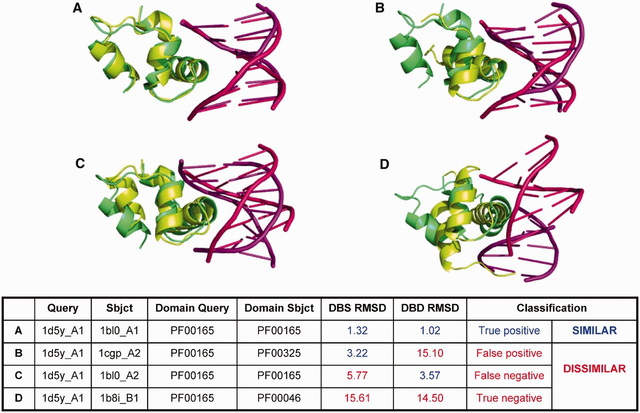
\includegraphics{tfcompare}
\caption%[]
{
Superposiciones de dominios de uni\'{o}n a DNA (DBD) de factores de transcripci\'{o}n, que ponen de manifiesto 
su mecanismo, no siempre conservado, de reconocimiento de sus cis-elementos (DBS). 
Figura tomada de \citet{Sebastian2013}.
}
\label{fig:tfcompare}
\end{center}
\end{figure}

Hay disponibles muchos otros programas disponibles para la comparaci\'{o}n estructural de prote\'{i}nas, 
y cada usuario tiene el suyo preferido. A qu\'{e} se debe esto? 
La raz\'{o}n es que no existe una definici\'{o}n totalmente satisfactoria del alineamiento estructural correcto, 
que es en definitiva la funci\'{o}n que todos estos algoritmos tratan de optimizar. De hecho, ni siquiera
est\'{a} claro si las taxonom\'{i}as estructurales cl\'{a}sicas, 
como \htmladdnormallink{CATH}{http://www.cathdb.info} o
\htmladdnormallink{SCOP}{http://scop.berkeley.edu} \citep{Csaba2009},
son compatibles con la evidencia disponible sobre la evoluci\'{o}n de los plegamientos (\italics{folds}), que
actualmente se imagina como un proceso discreto s\'{o}lo hasta cierto punto \citep{Taylor2002,Pascual2009,Sadowski2010,Andreeva2014}. 
De hecho \htmladdnormallink{SCOP2}{http://scop2.mrc-lmb.cam.ac.uk/} se hizo para superar esas limitaciones.
Otra complicaci\'{o}n adicional es que algunos plegamientos pueden verse como permutaciones circulares de elementos de estructura 
secundaria de otros \citep{Schmidt-Goenner2010}.

A pesar de estas dificultades, en general aceptamos que cada superfamilia de prote\'{i}nas es un \textbf{cl\'{u}ster}
de estructuras muy similares, que se pueden superponer aunque su secuencia sea muy diferente, 
y que cada plegamiento es un subconjunto de superfamilias que comparten una topolog\'{i}a de estructura secundaria.

Lo habitual cuando se publica un nuevo m\'{e}todo es compararlo con otros preexistentes. Estas comparaciones, 
si son rigurosas y reproducibles, pueden ayudar en la tarea de seleccionar un programa id\'{o}neo 
para esta tarea. El algoritmo MAMMOTH, con el que vamos a trabajar, se resume en estos pasos, 
en palabras textuales de sus autores \citep{Ortiz2002}:
\begin{quote}
 1.- From the Calpha trace,  compute the unit-vector  U-RMS  between
 all pairs of heptapeptides of both model and experimental structure.
 The  U-RMS is  described  in:  Kedem, Chew & Elber  (1999)  Proteins
 37(4):554-64,  and  in  Chew, Huttenlocher, Kedem & Kleinberg (1999)
 J.Comp.Biol. 6, 313-325.  This is a measure sensitive  to  the local
 structure.

  2.- Use the matrix derived in step 1 to find and alignment of local
 structures that maximizes the local similarity of both the model and
 the  experimental structure. For that, use a global alignment method 
 with  zero  end  gaps,  as  described  in  Needleman & Wunsch (1970) 
 J.Mol.Biol. 48, 443-453.

  3.- Find the maximum subset of similar  local  structures that have
 their corresponding  Calphas  close  in  cartesian space. "Close" is
 considered here  as  a distance less or equal than 4.0 A. The method
 to  find this subset is a small variant of the MaxSub algorithm from
 the  Fischer  group:  Siew,  Elofsson,  Rychlewski  & Fischer (2000)
 Bioinformatics, in press.

  4.- Obtain  the  probability  of  obtaining the given proportion of
 aligned residues (with respect to the  shortest  protein  model)  by
 chance.  This  metric  (E-value) is then used as the final score (or 
 the  corresponding Z-score, both are equivalent for gaussian distri-
 butions, however the Z-score is a more manegable index). In order to
 obtain this  value, an approach similar to that of Levitt & Gerstein 
 (1998) PNAS 95, 5913 is used, as  described  in  Abagyan  &  Batalov 
 (1997) J.Mol.Biol. 273, 355-368.  The E-value estimation is based on
 extreme-value fitting.  In  a  test  set  with the SCOP database, it 
 shows rather good performance.
\end{quote}
 
MAMMOTH fue comparado con varios m\'{e}todos, como se ve en esta figura:  

\begin{figure}
%\htmlimage{scale=0.5}
\begin{center} 
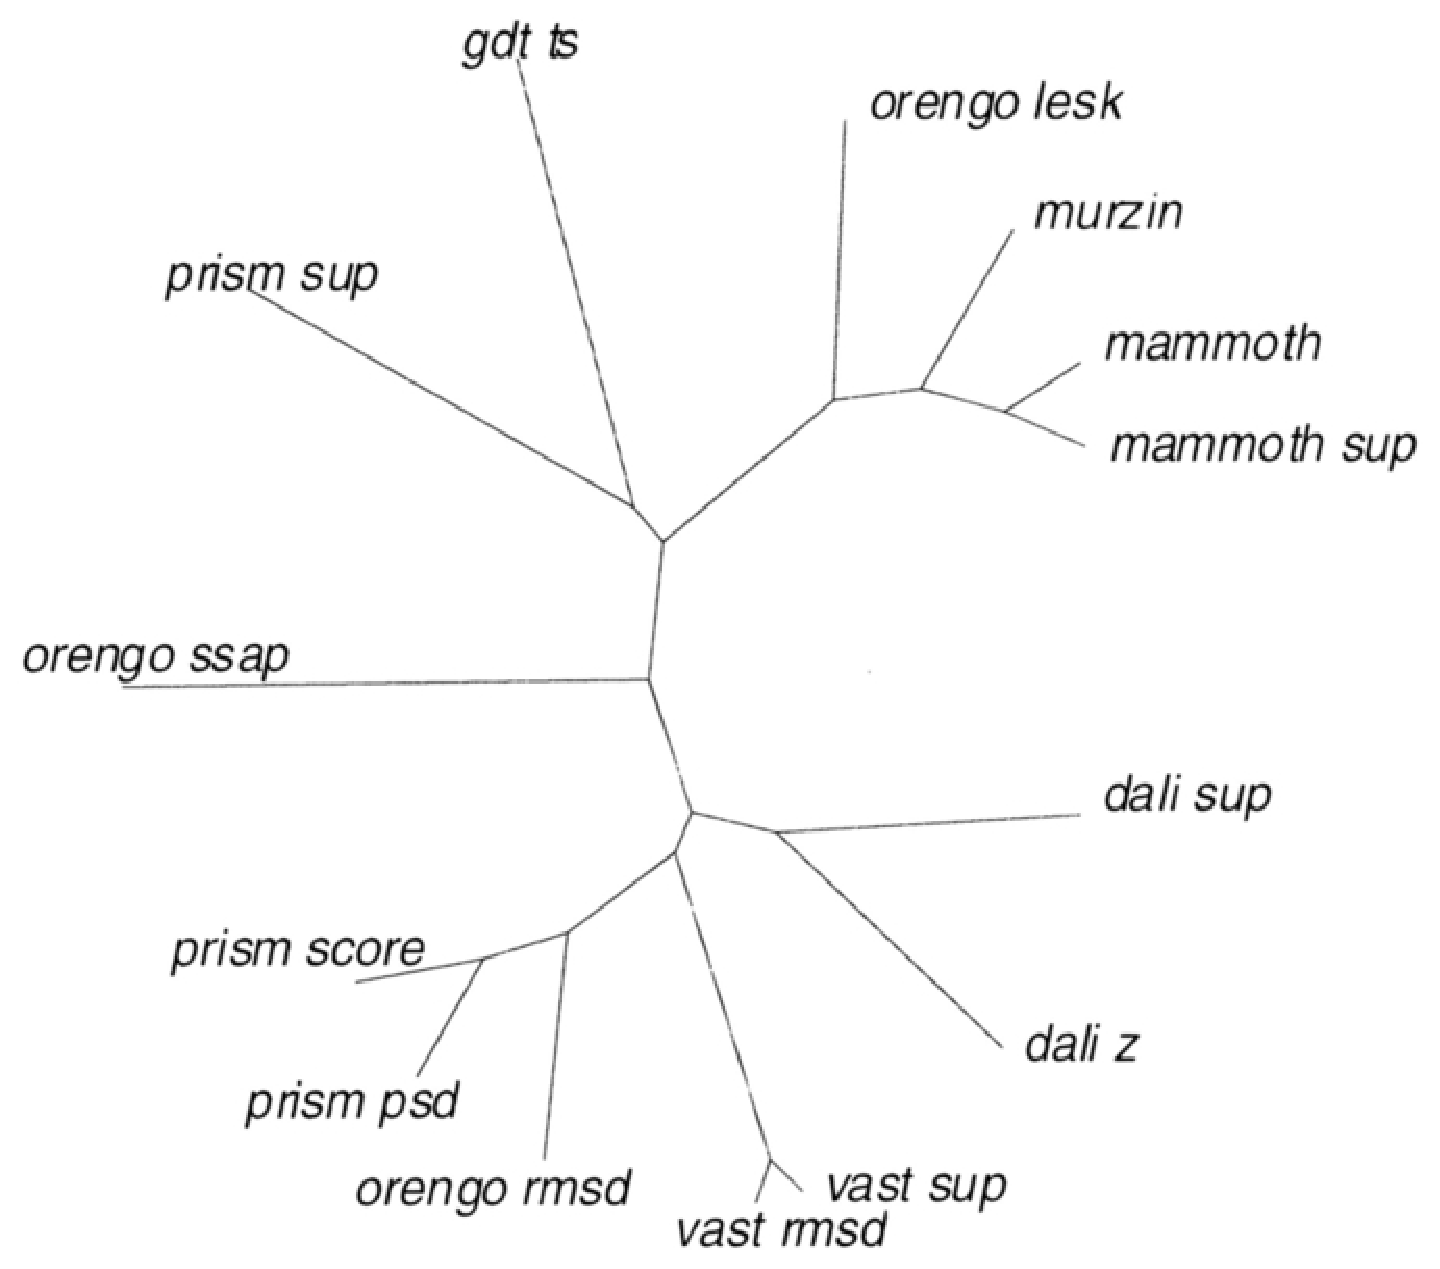
\includegraphics{mammoth_bench}
\caption%[]
{
Semejanza de MAMMOTH respecto a otros algoritmos de comparaci\'{o}n de estructura de prote\'{i}nas, 
incluyendo el criterio de un experto humano (Murzin). Figura tomada de \citet{Ortiz2002}. Copyright (2002) Protein Science.
}
\label{fig:mammoth}
\end{center}
\end{figure}
%$https://www.ncbi.nlm.nih.gov/pmc/articles/PMC2373724/

MAMMOTH es junto con DALI de los mejores programas, porque adem\'{a}s de generar superposiciones y alineamientos satisfactorios, 
sus medidas num\'{e}ricas de similitud devuelven valores que se ajustan a la evaluaci\'{o}n visual de la superposici\'{o}n obtenida.
En concreto, MAMMOTH devuelve para cada alineamiento una puntuaci\'{o}n y su valor esperado asociado (\italics{E-value}),
que podemos interpretar de manera an\'{a}loga a los valores esperados de BLAST, superando las limitaciones del RMSD para 
comparar estructuras que solamente se parecen en algunas regiones \citep{Siew2000}. 
Adem\'{a}s, hay una versi\'{o}n de MAMMOTH que permite calcular 
\htmladdnormallink{alineamientos m\'{u}ltiples}{https://ub.cbm.uam.es/software/mammothm.php}.

Para superar las limitaciones del RMSD, que da el mismo peso a regiones del core que a regiones divergentes, 
\citet{Zhang2004} propusieron otra funci\'{o}n, el TM-score, que disminuye el peso de las parejas alineadas a mayor distancia, es menos sensible
a la longitud de las estructuras comparadas y toma valores entre 0 y 1: 

\begin{equation}
TMscore = max[  \frac{1}{L_{Q}}  \sum_{i=1}^{L_{T}} \frac{1}{ 1 + (\frac{d_{i}}{d_{0}})^{2} } ]
\end{equation} 

Aqu\'{i} $max$ es el valor m\'{a}ximo obtenido en todas las superposiciones calculadas, 
$L_{Q}$ es la longitud de la estructura Q o \italics{query}, 
$L_{T}$ es el total de residuos alineados a la estructura T o \italics{template}, 
$d_{i}$ es la distancia entre la pareja $i$ de residuos y 
$d_{0}$ el factor de escala para normalizar por longitud de secuencia. 

Para calcularlo de manera \'{o}ptima podemos usar su algoritmo TM-align \citep{Zhang2005}, cuyo c\'{o}digo fuente esta disponible en 
\htmladdnormallink{TMalignc.tar.gz}{http://zhanglab.ccmb.med.umich.edu/TM-align/TM-align-C/TMalignc.tar.gz}. La funci\'{o}n TM-score
se ha convertido en el est\'{a}ndar para medir el parecido entre estructuras, ya que se acepta que un valor de 0.5 garantiza un plegamiento similar.

De todos modos, hay una gran variedad de software para esta tarea, 
como se muestra por ejemplo en esta \htmladdnormallink{lista de la WikipediA}{http://en.wikipedia.org/wiki/Structural_alignment_software}.

%\subsection{Ejercicios de similitud estructural entre estructuras proteicas con MAMMOTH}
Para aprender a hacer alineamientos/superposiciones estructurales, y a interpretarlos, podemos hacer este ejercicio:

\begin{itemize}

\item Visita \htmladdnormallink{SCOPe}{http://scop.berkeley.edu}, 
elige una clase (ver figura \ref{fig:foldclassif})
%elige la opci\'{o}n \italics{Enter SCOP at the top of the hierarchy} 
y selecciona un grupo de 5 estructuras de prote\'\i{}nas que pertenezcan a la misma superfamilia, para despu\'{e}s
\begin{itemize}
\item descargar los archivos PDB correspondientes,que contienen las coordenadas at\'{o}micas,  del
\htmladdnormallink{Protein Data Bank}{http://www.rcsb.org/pdb} y
\item compara al menos una pareja de estructuras con MAMMOTH %\htmladdnormallink{MAMMOTH}{https://ub.cbm.uam.es/software/mammoth.php} 
e inspecciona los archivos de salida generados (\verb+maxsub_sup.pdb,maxsub_sup2.pdb,rasmol.tcl+)
%o con la versi\'{o}n \htmladdnormallink{web}{https://ub.cbm.uam.es/software/online/mammoth.php})
\item (el ejecutable se encuentra en \verb+/home/compu2/algoritmos3D/soft/mammoth-1.0-src+)
\end{itemize}
 
\item Visualiza la superposici\'{o}n generada,  con Rasmol (usando la opci\'{o}n \verb+ -script rasmol.tcl+) y con PyMOL

\item Puedes probar a superponer estructuras directamente en \htmladdnormallink{PyMOL}{https://pymol.org/dokuwiki/doku.php?id=command:align}

\item Prueba MAMMOTH con el fin de comparar una estructura problema (una de las 5) contra una biblioteca
de estructuras en formato PDB (las otras 4), como si fuera BLAST. Cu\'{a}l de las 4 estructuras ser\'{i}a el mejor molde o \italics{template})
Cu\'{a}l es el l\'{i}mite esperado de precisi\'{o}n, en t\'{e}rminos de RMSD, que alcanzar\'{i}amos con cada molde?

\item Calcula para algunas de las superposiciones el \htmladdnormallink{TM-score}{http://zhanglab.ccmb.med.umich.edu/TM-score/}.

%Por ejemplo puedes comparar la luciferasa bacteriana 
%\htmladdnormallink{LuxA}{http://www.rcsb.org/pdb/explore/explore.do?structureId=1LUC} con las entradas de la
%biblioteca que puedes descargar de este \htmladdnormallink{enlace}{./files/scoplibrary.tgz} (3.7Mb).
\end{itemize}
\section{\italics{Protein fold recognition}} \label{FRsection}

Al analizar secuencias gen\'{o}micas frecuentemente encontraremos marcos de lectura (te\'{o}ricos) que codifican para prote\'{i}nas que aparentemente no se parecen a ninguna otra (llamadas a veces \italics{orphans} en la literatura), 
o que s\'{o}lo tienen similitudes obvias con prote\'{i}nas de funci\'{o}n desconocida. Esto puede deberse a que de veras son 
mol\'{e}culas observadas por primera vez, o como vimos en \ref{threedeecons}, a que la evoluci\'{o}n ha conservado en mayor grado
la estructura y topolog\'{i}a de las prote\'{i}nas hom\'{o}logas que sus secuencias. 

La segunda posibilidad ha justificado una familia de m\'{e}todos llamados gen\'{e}ricamente de \italics{Fold Recognition} (FR), 
que tienen como objeto reconocer a qu\'{e} tipo de plegamiento (de los conocidos) se debe asignar una secuencia problema, 
especialmente cuando b\'{u}squedas m\'{a}s convencionales con 
\htmladdnormallink{BLAST}{http://blast.ncbi.nlm.nih.gov/Blast.cgi} o 
\htmladdnormallink{FASTA}{http://www.ebi.ac.uk/Tools/fasta/index.html}
han fracasado.
Hist\'{o}ricamente algunos de estos m\'{e}todos se han llamado de
\htmladdnormallink{\italics{threading}}{http://en.wikipedia.org/wiki/Threading_\%28protein_sequence\%29}, 
ya que ciertos algoritmos 
literalmente enhebran la secuencia problema en patrones de coordenadas conocidas, normalmente un subconjunto no redundante
del PDB, para ver si es compatible con alguno, como en la siguiente figura:

\begin{figure}
\begin{center} 
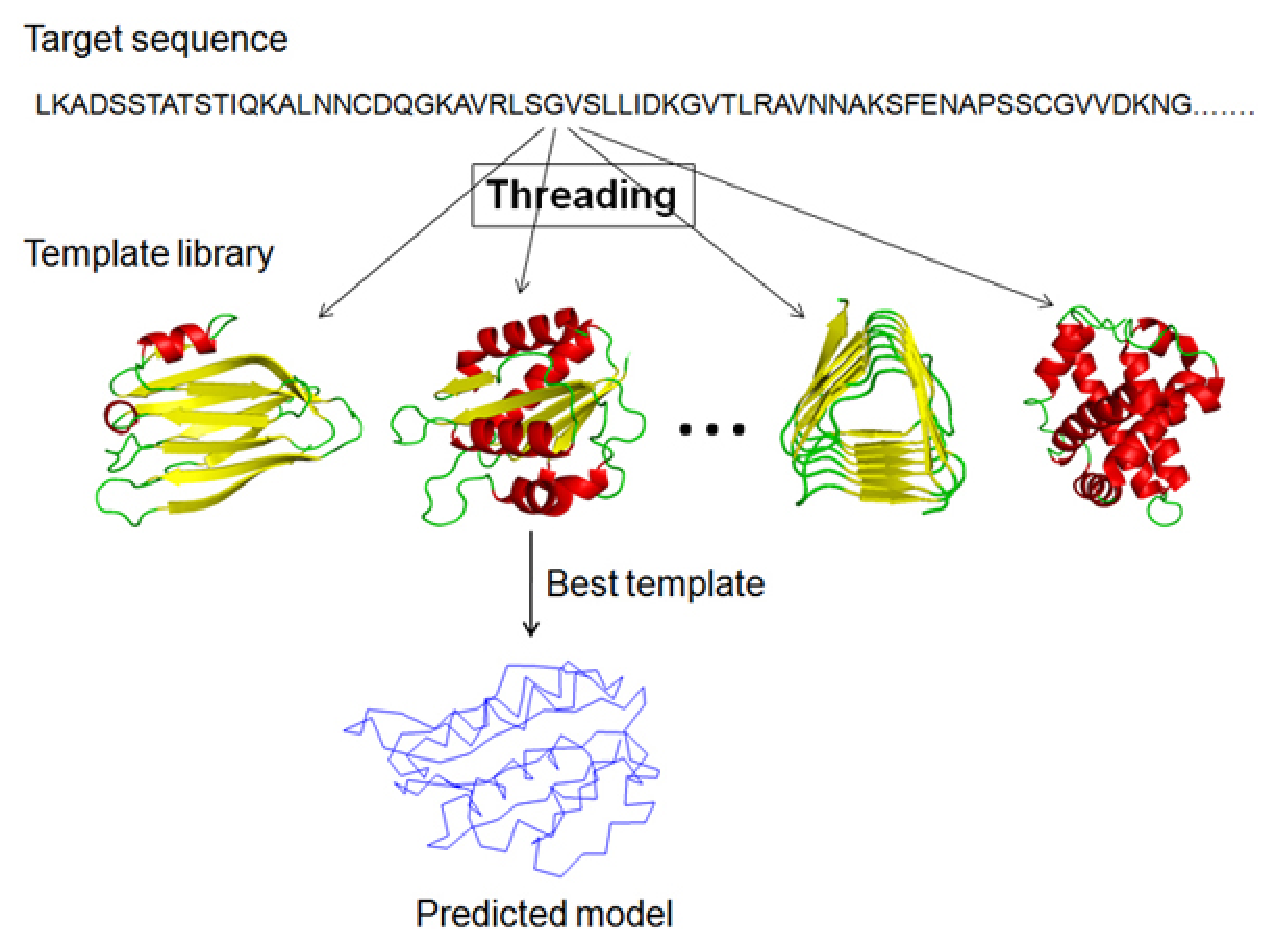
\includegraphics{threading}
\caption%[]
{
Diagrama de flujo de los algoritmos de reconocimiento de plegamiento (FR).
Figura tomada de \cite{Guo2008}. Copyright (2008) Frontiers in Bioscience. 
}
\label{fig:threading}
\end{center}
\end{figure}

El problema de FR lo podemos plantear as\'{i}:
\begin{itemize}
\item \textbf{PROBLEMA:} conocemos la secuencia de una prote\'{i}na, pero desconocemos su tipo de plegamiento y su funci\'{o}n
\item \textbf{SOLUCI\'{O}N PROPUESTA:} comparar la secuencia con todos los plegamientos conocidos, calcular el grado de parecido/compatibilidad con cada uno de ellos y devolver una lista ordenada
\end{itemize}

Se han publicado muchos algoritmos diferentes de FR; en todos ellos de alguna manera se asigna una estructura T a una secuencia A:
\begin{itemize}
\item Por medio de b\'{u}squedas PSI-BLAST bidireccionales transitivas \citep{Koretke2002}. 
La idea es que si buscamos secuencias hom\'{o}logas a partir de A llegamos a encontrar, en alguna iteraci\'{o}n, 
la secuencia T entre los resultados con cierta significancia estad\'{i}stica. De la misma manera, a partir de la secuencia de T llegamos a la secuencia A.

%(\htmladdnormallink{Pubmed}{http://www.ncbi.nlm.nih.gov/pubmed/12021456})
\item Representando cada plegamiento o \italics{fold} por medio de las secuencias conocidas que se pliegan en esa conformaci\'{o}n
y comparten estructura secundaria. Esto se puede hacer por medio de perfiles de secuencia \citep{Gribskov1987}, 
que son matrices sustituci\'{o}n de amino\'{a}cidos espec\'{i}ficas de posici\'{o}n, 
%\htmladdnormallink{perfiles}{http://www.ncbi.nlm.nih.gov/pubmed/3474607} 
o \htmladdnormallink{modelos ocultos de Markov}{http://en.wikipedia.org/wiki/Hidden_Markov_model}, 
que modelan expl\'{i}citamente con qu\'{e} probabilidad se pueden emitir secuencias compatibles con ese plegamiento.

\item Por medio de alineamientos secuencia-perfil %\htmladdnormallink{secuencia-perfil}{http://www.ncbi.nlm.nih.gov/pubmed/12169530} 
o los m\'{a}s sensibles perfil-perfil \citep{Soding2005} %\htmladdnormallink{perfil-perfil}{http://www.ncbi.nlm.nih.gov/pubmed/15531603}, 
que son la raz\'{o}n del \'{e}xito del servidor \htmladdnormallink{HHpred}{https://toolkit.tuebingen.mpg.de/#/tools/hhpred}.

\item Usando potenciales estad\'{i}sticos para evaluar la cercan\'{i}a de los residuos de una secuencia
dado un plegamiento (lo que llamamos \italics{threading} \citep{Threader1992}). Estos m\'{e}todos requieren precalcular,
sobre una colecci\'{o}n de plegamientos no redundantes, con qu\'{e} frecuencia y a qu\'{e} distancia se forman 
parejas de residuos en las estructuras conocidas. %(\htmladdnormallink{genTHREADER}{http://www.ncbi.nlm.nih.gov/pubmed/10191147})

%\item ombinando diferentes moldes, alineamientos y algoritmos en estrategias de b\'{u}squeda de consenso, 
%con la ayuda de m\'{e}tricas fiables como \htmladdnormallink{3D-Jury}{http://www.ncbi.nlm.nih.gov/pmc/articles/PMC2040163/} \citep{Ginalski2003}

%\item Partiendo la secuencia problema en fragmentos, como una estrategia divide y vencer\'{a}s, buscando la estructura
%mas probable para cada fragmento por \italics{threading} \citep{Wu2010}

\end{itemize}

Probablemente la mejor manera de evaluar objetivamente y elegir un m\'{e}todo de FR 
son experimentos colectivos a ciegas con secuencias cuyas estructuras experimentales se hacen p\'{u}blicas
tras las entrega de las predicciones. Hay dos tipos de experimentos de estipo: 
\htmladdnormallink{CASP}{http://predictioncenter.org/index.cgi?page=public_serv}, 
que mide bianualmente la competencia de los algoritmos de los grupos participantes, y 
\htmladdnormallink{CAMEO}{https://www.cameo3d.org}, que hace evaluaciones continuas no supervisadas.

En palabras de \citet{Kelley2015}, desarrollador principal de 
\htmladdnormallink{Phyre2}{http://www.sbg.bio.ic.ac.uk/phyre2}, uno de los m\'{a}s completos,
los mejores predictores tienen resultados indistinguibles en la mayor parte de los casos,
pero en los casos mas complejos desde hace tiempo destaca por su consistencia y 
superiores resultados \htmladdnormallink{I-TASSER}{http://zhanglab.ccmb.med.umich.edu/I-TASSER}.

%En la pr\'{a}ctica, a menudo los usuarios recurrimos a
%\htmladdnormallink{metaservidores}{http://en.wikipedia.org/wiki/Metaserver} como
%\htmladdnormallink{BioInfobank}{http://meta.bioinfo.pl}, desde donde podemos mandar una secuencia problema 
%a muchos servidores de FR, y lo que es m\'{a}s importante, donde podemos evaluar de una manera fiable 
%la calidad de los resultados usando m\'{e}tricas basadas en consensos, como 
%%\htmladdnormallink{2003}{http://bioinformatics.oxfordjournals.org/cgi/reprint/19/8/1015} y 
%\htmladdnormallink{3D-Jury}{http://www.ncbi.nlm.nih.gov/pmc/articles/PMC2040163/} \citep{Ginalski2003}, 
%como podemos comprobar inspeccionando la \htmladdnormallink{tabla de resultados}{http://meta.bioinfo.pl/queue.pl} de BioInfobank.

Estas herramientas web son adecuadas para estudiar unas pocas secuencias, pero si queremos hacer un experimento de FR 
a gran escala, entonces buena idea instalar localmente el software elegido, como por ejemplo
\htmladdnormallink{hh-suite}{https://github.com/soedinglab/hh-suite}, el software que da vida a 
\htmladdnormallink{HHpred}{https://toolkit.tuebingen.mpg.de/#/tools/hhpred}.

El siguiente programa es un prototipo de alineamiento perfil-perfil que usa adem\'{a}s predicciones de estructura secundaria (ver figura \ref{fig:psipred}) 
para guiar el alineamiento. Es un algoritmo de programaci\'{o}n din\'{a}mica, que puedes comprender mejor con ayuda 
del \htmladdnormallink{\italics{Sequence Alignment Teacher}}{http://protein.bio.puc.cl/websoftware/web/?sid=3} \citep{Ibarra2010}.

Para probarlo necesitaras descargar los archivos de entrada
(\htmladdnormallink{1ngk\_A.pssm}{./files/1ngk_A.pssm},
\htmladdnormallink{1s69\_A.pssm}{./files/1s69_A.pssm},
\htmladdnormallink{1ngk\_A.psipred}{./files/1ngk_A.psipred},
\htmladdnormallink{1s69\_A.psipred}{./files/1s69_A.psipred}):
\verbatiminput{code/prog3.2.pl}
\section{Modelado de prote\'\i{}nas por homolog\'{i}a} \label{CM}

Con las herramientas que hemos estado manejando ya estamos preparados para modelar prote\'\i{}nas. 
En este contexto modelar significa hacer una predicci\'{o}n de c\'{o}mo se disponen los \'{a}tomos 
de una prote\'\i{}na conocida su secuencia, con el fin de estudiar su funci\'{o}n molecular, su historia evolutiva o, 
si el modelo es bueno, dise\~nar o muestrear ligandos e incluso calcular sus afinidades \citep{Singh2010}. 
Asimismo este tipo de modelos se usan mucho para estudiar el efecto de mutaciones puntuales \citep{Kellogg2011}.

\begin{itemize}
\item \textbf{PROBLEMA:} disponemos de la secuencia de una prote\'{i}na A y quisi\'{e}ramos conocer, aunque sea de manera aproximada, 
su estructura tridimensional
\item \textbf{SOLUCI\'{O}N PROPUESTA:} estimar coordenadas cartesianas para la mayor\'{i}a de los \'{a}tomos de A, 
en base a la estructura conocida de prote\'{i}nas  similares, que llamamos plantillas, moldes, o \italics{templates}
\end{itemize}

Esta metodolog\'{i}a se llama modelado comparativo o por homolog\'{i}a y se describe en profundidad en este
art\'\i{}culo de \citet{Fiser2003}. %\htmladdnormallink{art\'\i{}culo}{./papers/modeller2003.pdf} 
Hay fundamentalmente dos estrategias, que en general requieren alineamientos entre la secuencia problema y los posibles moldes:
\begin{itemize}

\item Ensamblaje de grandes fragmentos r\'{i}gidos, incluso el plegamiento entero, 
obtenidos de estructuras similares alineadas por medio de su secuencia primaria y secundaria
(\htmladdnormallink{SWISS-MODEL}{http://swissmodel.expasy.org}, 
\htmladdnormallink{IntFOLD}{http://www.reading.ac.uk/bioinf/IntFOLD}, 
\htmladdnormallink{ROBETTA}{http://robetta.bakerlab.org} o 
%\htmladdnormallink{3D-JIGSAW}{http://bmm.cancerresearchuk.org/~3djigsaw} 
\htmladdnormallink{MEDELLER}{http://opig.stats.ox.ac.uk/webapps/medeller/home.pl?app=MEDELLER} para prote\'{i}nas transmembrana).
Esta metodolog\'{i}a corta y pega literalmente fragmentos del esqueleto pept\'{i}dico de estructuras conocidas.

\item Modelado por satisfacci\'{o}n de restricciones (distancias, \'{a}ngulos) moleculares extra\'{i}das 
de bases de datos y estructuras similares alineadas (\htmladdnormallink{MODELLER}{https://salilab.org/modeller/}). 
Este m\'{e}todo, conceptualmente similar a la resoluci\'{o}n por NMR (ver secci\'{o}n \ref{metodosExp}), 
produce un conjunto de estructuras para la secuencia A, 
todas ellas compatibles con las restricciones observadas en los \italics{templates}.

\end{itemize}

El algoritmo gen\'{e}rico de modelado comparativo puede dividirse en varios pasos, ilustrados en la figura \ref{fig:CMflow}:
\begin{itemize}
\item{1.} Identificar por similitud de secuencia dominios $D_{1..d}$ en la prote\'\i{}na $S$ que queremos modelar.
\item{2.} Buscar y alinear estructuras molde $M_{1..m}$ que nos sirvan para modelar uno o m\'{a}s dominios de $S$. 
Cada dominio con al menos un molde es potencialmente modelable.
\item{3.} Para cada dominio $D_{i}$ modelable:
\begin{itemize}
\item{3.1.} Refinar el alineamiento local de cada segmento alineado del molde.
\item{3.2.} Tomar las coordenadas pept\'{i}dicas (o descriptores moleculares) de la estructura molde alineada.
\item{3.3.} Copiar los \htmladdnormallink{rot\'{a}meros}{http://kinemage.biochem.duke.edu/databases/rotamer.php}
de las cadenas laterales de los amino\'{a}cidos conservados en el alineamiento.
\item{3.4.} Modelar los rot\'{a}meros de los residuos que mutan respecto al molde, 
con ayuda de una \htmladdnormallink{biblioteca}{http://dunbrack.fccc.edu/bbdep2010}.
\begin{figure}
\begin{center} 
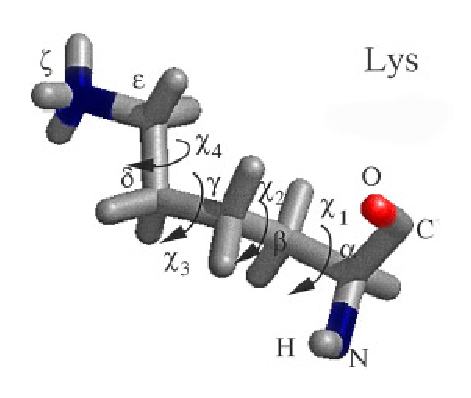
\includegraphics{rotamer}
\caption%[]
{
\'{A}ngulos que definen los rot\'{a}meros de las cadenas laterales.
%figura tomada de \htmladdnormallink{http://bopwww.biologie.uni-freiburg.de}{http://bopwww.biologie.uni-freiburg.de/students/labs/synopsis_jul02/index.html}.
}
\label{fig:rotamer}
\end{center}
\end{figure}
\item{3.4.} A\~nadir los segmentos, normalmente \htmladdnormallink{\italics{loops}}{http://bmm.cancerresearchuk.org/loop}, 
correspondientes a \italics{gaps} en la secuencia alineada del molde.
\item{3.5.} Refinar 1 \'{o} m\'{a}s modelos completos $P_{n}$ con el objeto de eliminar errores obvios de estructura, como impedimentos o choques est\'{e}ricos.
\item{3.6.} Evaluar los modelos $P_{n}$  y estimar su calidad, por medio de aplicaciones como 
\htmladdnormallink{ProQ3}{http://proq3.bioinfo.se},
\htmladdnormallink{Verify3D}{http://services.mbi.ucla.edu/Verify_3D} o 
\htmladdnormallink{FiltRest3D}{http://filtrest3d.genesilico.pl/filtrest3d/index.html}.
\end{itemize}
\end{itemize}

El paso 2 es el m\'{a}s determinante sobre la calidad del modelo y de hecho marca el techo de precisi\'{o}n de la metodolog\'{i}a 
\citep{ContrerasMoreira2005}. Es adem\'{a}s un paso cr\'{i}tico en el sentido de que si el alineamiento $M_{i}$ es malo, 
el modelo resultante ser\'{a} malo, como ya vislumbramos en la secci\'{o}n \ref{threedeecons}. Para modelos complicados ser\'{a} 
necesario explorar diferentes combinaciones de moldes y alineamientos para encontrar la mejor soluci\'{o}n. %\citep{Contreras-Moreira2003}.
Si la secuencia problema es multidominio o multim\'{e}rica puede ser necesario modelar su estructura cuaternaria \citep{Tramontano2017}, 
con herramientas especiales como
\htmladdnormallink{BAM}{http://dunbrack.fccc.edu/BAM} o 
\htmladdnormallink{AIDA}{http://ffas.burnham.org/AIDA}.

Con el objeto de explicar en mayor detalle el algoritmo, el siguiente c\'{o}digo implementa los pasos 3.1 y 3.2, quiz\'{a}s
los m\'{a}s fundamentales tras el el paso 2. El programa usa como ejemplo secuencias
y estructuras ya utilizadas en el apartado \ref{threedeecons} (\htmladdnormallink{1gd6.pdb}{./files/1gd6.pdb}):
\verbatiminput{code/prog3.3.py}

Como en otros campos de la biolog\'{i}a computacional, el repertorio de software para modelar prote\'{i}nas es muy extenso,
y constantemente incluye nuevas herramientas que sustituyen a otras que envejecen.
Un buen punto de partida para elegir la mejor soluci\'{o}n son los \italics{rankings} que actualiza cada dos a\~nos 
\htmladdnormallink{CASP}{http://predictioncenter.org/index.cgi?page=public_serv}, aunque probablemente los 
programas de modelado preferidos por los usuarios son SWISS-MODEL en la Web y MODELLER como instalable.

\begin{figure}
%\htmlimage{scale=0.5}
\begin{center} 
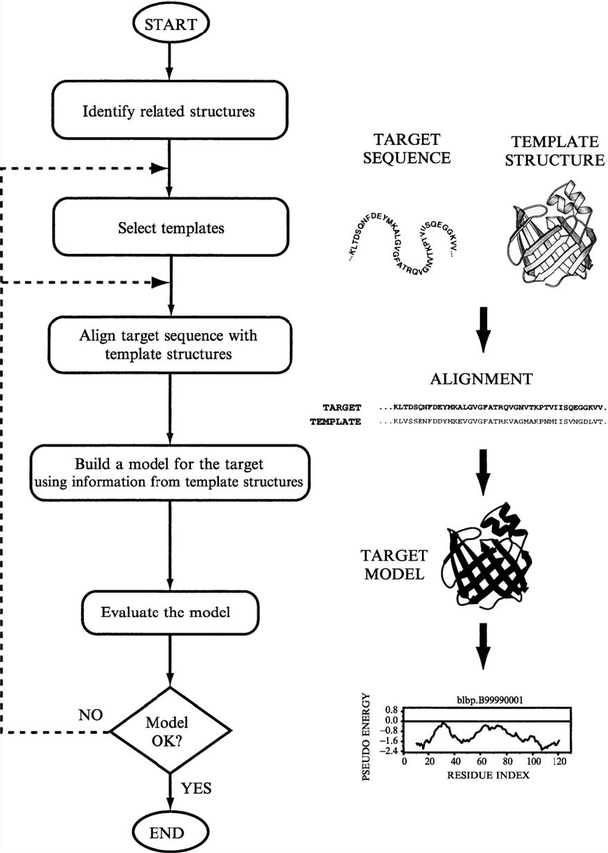
\includegraphics{CMflow}
\caption%[]
{
Algoritmo gen\'{e}rico de modelado comparativo.
Figura tomada de \citet{Fiser2003}. Copyright (2003) Methods in Enzymology.
}
\label{fig:CMflow}
\end{center}
\end{figure}

\begin{figure}
\begin{center} 

\includegraphics{figure_3_contrera_review_final}
\caption%[]
{
Los errores en modelado comparativo se disparan al usar estructuras molde con identidades bajas.
Este comportamiento se observa con diferentes herramientas de modelado, incluyendo SWISS-MODEL.
Figura de \citet{Contreras-Moreira2002b}. 
}
\label{fig:CMbench}
\end{center}
\end{figure}

En la pr\'{a}ctica podemos hacer nuestros modelos por homolog\'{i}a, con la opci\'{o}n de controlar todos los pasos
del procedimiento, por medio del programa \htmladdnormallink{MODELLER}{https://salilab.org/modeller} \citep{Sali1993}, 
disponible sin costo para usuarios acad\'{e}micos. %\verb+/home/bioinfo/bin/modeller8v1/bin/mod8v1+ 
El programa tiene \htmladdnormallink{m\'{u}ltiples posibilidades}{https://salilab.org/modeller/tutorial/}, pero en este ejemplo
nos centramos en el caso m\'{a}s sencillo consistente en hacer un modelo a partir de un s\'{o}lo molde o \italics{template},
estimando su calidad del modelo por medio de la funci\'{o}n DOPE \citep{Shen2006}:
\begin{itemize}

\item Secuencia problema: \htmladdnormallink{FNR}{http://www.expasy.org/uniprot/FNR_ECOLI}, 
regulador transcripcional de \italics{Escherichia coli}.

\item Busca, por ejemplo usando PSI-BLAST, secuencias similares (probablemente hom\'{o}logas)
cuya estructura est\'{e} en el PDB (moldes o \italics{templates}).

\item Para cada uno de los \italics{templates} interesantes sigue estos pasos:
\begin{itemize}

	\item descarga el fichero de coordenadas del \htmladdnormallink{PDB}{http://www.rcsb.org/pdb} 
	y extrae la secuencia S contenida en los campos \verb+ATOM+

	\item alinea la secuencia S de las coordenadas con la secuencia problema (FNR, por ejemplo con 
  \htmladdnormallink{clustal-omega}{https://www.ebi.ac.uk/Tools/msa/clustalo} o usando el mismo alineamiento de BLAST) 
	y crea un archivo con extensi\'{o}n 
	\verb+.ali+ con este formato, donde \verb+structureX+ es el molde, \verb+sequence+ es la secuencia problema o \italics{query} 
	y los dem\'{a}s campos definen el rango de residuos alineados del \italics{template}, y su resoluci\'{o}n:

\begin{verbatim}
C; Alineamiento de muestra en formato PIR
>P1;1PDB
structureX:1PDB:1    :A:106  :A:nombre_template:: 1.90: 
AFVVTDNCIKCKYTDCVEVCPVDCFYEGPNFLVIHPDECIDCALCEPECPAQAIFSEDEVPEDMQEFIQLNAELA
EVWPNITEKKDPLPDAEDWDGVKGKLQHLER*
>P1;query
sequence:query:::::::0.00: 0.00
AYVINDSC--IACGACKPECPVNIIQGS--IYAIDADSCIDCGSCASVCPVGAPNPED-----------------
-------------------------------*
\end{verbatim}

	\item genera un gui\'{o}n o \italics{script} para MODELLER como \verb+guion_nombre_template.py+:

\begin{verbatim}
from modeller.automodel import *   

log.verbose()    
env = environ() 

# 1) directorio donde se encuentran los ficheros con coordenadas de moldes/templates, 
# con extension .pdb,.atm,.ent
env.io.atom_files_directory = './templates/'

# 2) prepara el modelado
a = automodel(env,
              alnfile  = 'alineamiento.ali',  # fichero con el alineamiento
              knowns   = '1PDB',              # nombre del template como aparece en alnfile
              sequence = 'query',             # nombre de secuencia problema como aparece en alnfile
	          assess_methods=(assess.DOPE))      

a.starting_model= 1                           # define cuantos modelos diferentes quieres
a.ending_model  = 2                 
				  
# 3) accion! 
a.make()                  
\end{verbatim}

	\item ahora ejecuta MODELLER (por ejemplo poniendo en el terminal: \verb+$ mod9v8 guion_template.py+ y al terminar revisa 
	\verb+guion_nombre_template.log+ para comprobar la evaluaci\'{o}n emp\'{i}rica del modelo o modelos obtenidos

\end{itemize}
\end{itemize}


%%%%%%%%%%%%%%%%%%%%%%%%%%%%%%%%%%%%%%%%%%%%%%%%%%%%%%%%%%%%%%%%%%%%%%%%%%%%%%%
%%%%%%%%%%%%%%%%%%%%%%%%%%%%%%%%%%%%%%%%%%%%%%%%%%%%%%%%%%%%%%%%%%%%%%%%%%%%%%%


\section{Modelado de prote\'\i{}nas \italics{ab initio}} \label{abinitio}

Hablamos de protocolos \italics{ab initio} cuando tratamos de modelar
el plegamiento de un polip\'{e}ptido solamente a partir de su secuencia y de la f\'\i{}sica  \citep{Baker2001}. 
Sin embargo, los m\'{e}todos de este tipo
m\'{a}s exitosos hasta la fecha reconstruyen la estructura terciaria a base de peque\~{n}os fragmentos cortados 
de estructuras conocidas y seleccionados por similitud de secuencia. 

El mejor ejemplo es el algoritmo Rosetta \citep{Simons1997}, implementado en el servidor web 
\htmladdnormallink{ROBETTA}{http://robetta.bakerlab.org}, 
que permite modelar secuencias cortas cuando no hay moldes que alineen con la secuencia problema, 
ni siquiera por \italics{fold recognition} (ver secci\'{o}n \ref{FRsection}). 
Usa fragmentos de 9 amino\'{a}cidos de longitud. En este caso podemos definir el problema tipo de esta manera:

\begin{itemize}
\item \textbf{PROBLEMA:} disponemos de la secuencia de una prote\'{i}na A y quisi\'{e}ramos conocer, aunque esa de manera aproximada, su estructura tridimensional
\item \textbf{SOLUCI\'{O}N PROPUESTA:} combinar fragmentos tomados de estructuras del PDB, generar conformaciones alternativas y seleccionar las mejores
\end{itemize}

\begin{figure}
\begin{center} 
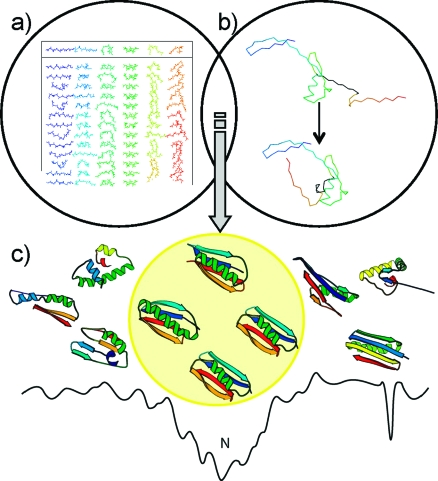
\includegraphics{rosetta}
\caption%[]
{
Resumen del protocolo Rosetta, tomado de \citet{Kaufmann2010}.
A) Se seleccionan de una biblioteca los fragmentos con secuencias mas parecidas a los $K$-meros de la secuencia problema ($K=9$).
B) Combinaci\'{o}n de fragmentos solapantes para generar muchas conformaciones alternativas.
C) Optimizaci\'{o}n de conformaciones con funciones que eval\'{u}an interacciones no locales. 
Copyright (2010) Biochemistry.
}
\label{fig:Rosetta}
\end{center}
\end{figure}

Este tipo de algoritmos requieren tener precalculada una biblioteca de fragmentos de longitud $K$ de estructura conocida,
funciones para seleccionar los mejores fragmentos para cada $K$-mero de la secuencia problema,
funciones de evaluaci\'{o}n que permitan descubrir conformaciones que se parezcan a las nativas, 
y muchos recursos computacionales, dado que todos estos pasos son costosos.
Otro algoritmo que funciona tanto para \italics{fold recognition} como para modelado \italics{ab initio} es 
\htmladdnormallink{I-TASSER}{http://zhanglab.ccmb.med.umich.edu/I-TASSER}:

\begin{figure}
\begin{center} 
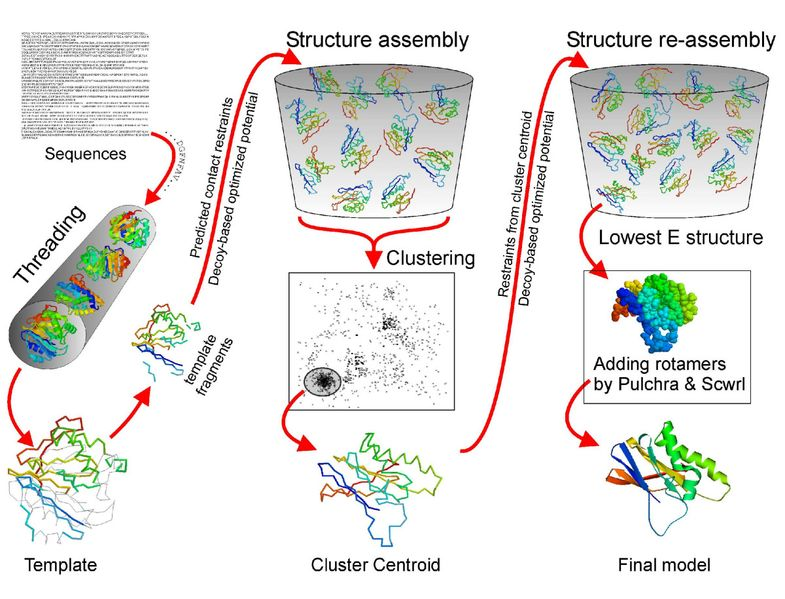
\includegraphics{ITASSER}
\caption%[]
{
Resumen del protocolo TASSER. 
Figura de \citet{Wu2007}, reproducida con permiso de los autores.
}
\label{fig:ITASSER}
\end{center}
\end{figure}
\section{Modelado de prote\'{i}nas por predicci\'{o}n de contactos} \label{contactosPred}

Las matrices de contactos (ver secci\'{o}n \ref{estr34})  han sido durante mucho tiempo una fuente de inspiraci\'{o}n de m\'{e}todos 
de predicci\'{o}n estructural, con la idea subyacente de 'si somos capaces de predecir con informaci\'{o}n evolutiva qu\'{e} residuos de 
una secuencia contactan, entonces podremos resolver su estructura' \citep{Gobel1994,deJuan2013}.

La informaci\'{o}n evolutiva en cuesti\'{o}n es normalmente un alineamiento m\'{u}ltiple de secuencias hom\'{o}logas, que se espera
capturen de forma impl\'{i}cita las limitaciones que impone la estructura terciaria de un dominio a las sustituciones de amino\'{a}cidos
que contactan. La funci\'{o}n matem\'{a}tica que se emplea habitualmente para estudiar esto es la 
\htmladdnormallink{informaci\'{o}n mutua}{http://es.wikipedia.org/wiki/Informaci\%C3\%B3n\_mutua} (MI), 
que mide la dependencia entre dos variables, en este caso columnas de un alineamiento.

\begin{figure}
\begin{center} 
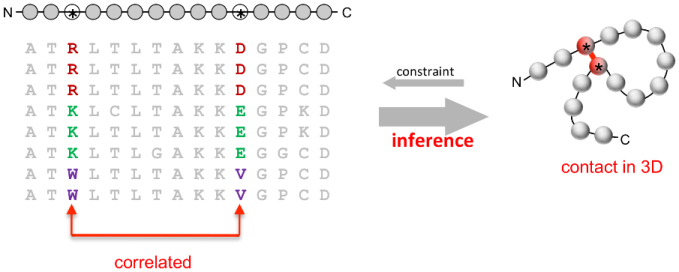
\includegraphics{EVfoldcorr}
\caption%[]
{
Las mutaciones correlacionadas entre columnas de un alineamiento m\'{u}ltiple se pueden emplear para predecir contactos entre residuos en el plegamiento.
Figura tomada de \cite{Marks2011} y reproducida con permiso de los autores.
}
\label{fig:EVfold1}
\end{center}
\end{figure}

Por tanto, el problema de la predicci\'{o}n de contactos se puede plantear as\'{i}:
\begin{itemize}
\item \textbf{PROBLEMA:} conocemos la secuencia de una prote\'{i}na y las de muchas secuencias hom\'{o}logas
\item \textbf{SOLUCI\'{O}N PROPUESTA:} alineamos las secuencias, buscamos posiciones que muestren evidencia de coevoluci\'{o}n 
y buscamos plegamientos compatibles con esos contactos
\end{itemize}

El algoritmo \htmladdnormallink{EVfold}{http://EVfold.org} %, publicado originalmente en \citep{Marks2011}, 
emplea estos elementos
para hacer predicciones de contactos de alta calidad, ya que es capaz de distinguir entre posiciones de la secuencia
que directamente contactan (causativas) de las que correlacionan simplemente porque contactan con un mismo residuo (transitivas). 
Usando su terminolog\'{i}a,
MI es un modelo local de probabilidad de contactos, que ellos son capaces de corregir y convertir en un modelo global usando conceptos 
de la mec\'{a}nica estad\'{i}stica y la maximizaci\'{o}n de la entrop\'{i}a. El modelo global se llama de Informaci\'{o}n Directa (DI)
\citep{Marks2011}.

\begin{figure}
\begin{center} 
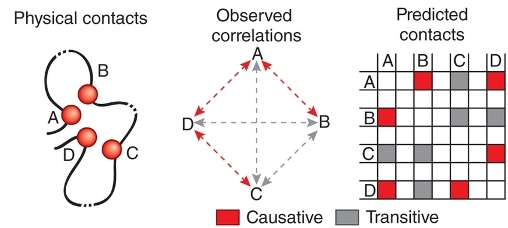
\includegraphics{EVfold22}
\caption%[]
{
Definici\'{o}n de contactos entre residuos (A,B,C,D) y de correlaciones directas y transitivas.
Figura tomada de \cite{Marks2012}. Copyright (2012) Nature Biotechnology.
}
\label{fig:EVfold1.1}
\end{center}
\end{figure} %https://www.ncbi.nlm.nih.gov/pmc/articles/PMC4319528/figure/F2/

\begin{figure}
\begin{center} 
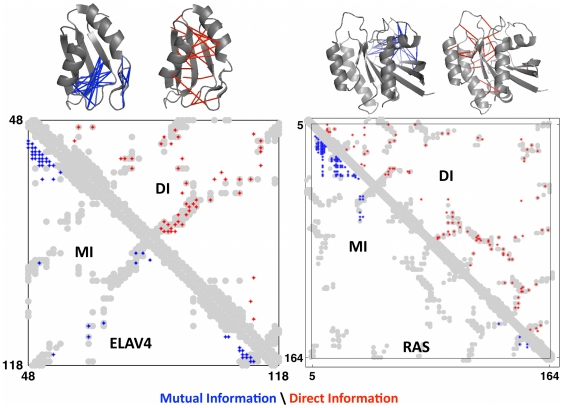
\includegraphics{EVfold3}
\caption%[]
{
La inferencia de contactos entre residuos es mejor con el modelo global (DI, ver texto) que con el modelo local MI.
La figura muestra predicciones de contactos para las prote\'{i}nas ELAV4 (derecha) y RAS (izquierda).
Las predicciones globales se reparten uniformemente por la secuencia y se solapan mejor con los contactos observados en estructuras experimentales.
Figura tomada de \cite{Marks2011} y reproducida con permiso de los autores.
}
\label{fig:EVfold2}
\end{center}
\end{figure}

La siguiente figura muestra el diagrama de flujo completo del m\'{e}todo \htmladdnormallink{EVfold}{http://EVfold.org}, 
que ha sido posteriormente adaptado para prote\'{i}nas transmembrana \citep{Hopf2012} y 
tambi\'{e}n para complejos cuaternarios \citep{Hopf2014}:

\begin{figure}
\begin{center} 
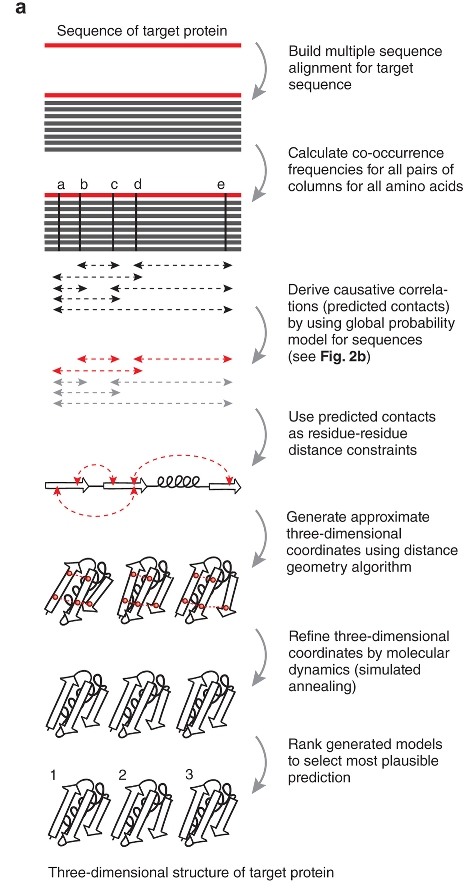
\includegraphics{EVfold21}
\caption%[]
{
Algoritmo de plegamiento de prote\'{i}nas en base a observaciones de mutaciones correlacionadas,
que se transforman en predicciones de contactos, tomado de \cite{Marks2012}. Copyright (2012) Nature Biotechnology.
}
\label{fig:EVfold3} %https://www.ncbi.nlm.nih.gov/pmc/articles/PMC4319528/figure/F2/
\end{center}
\end{figure}

La siguiente figura muestra los resultados de un experimento de validaci\'{o}n de EVfold:

\begin{figure}
\begin{center} 
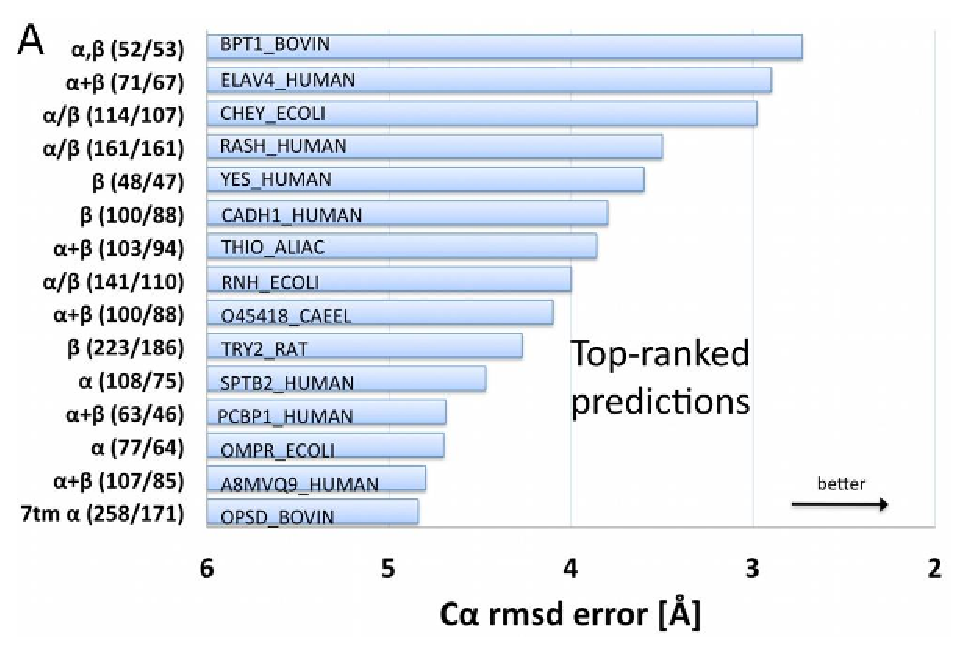
\includegraphics{EVfoldbenchA}
\caption%[]
{
Calidad de las mejores predicciones de EVfold en un conjunto de 15 prote\'{i}nas con diferentes composiciones de estructuras secundaria.
Entre par\'{e}ntesis se muestran el n\'{u}mero de residuos del dominio modelado y 
el n\'{u}mero de residuos sobre los que se calcul\'{o} el RMSD entre el modelo y la estructura experimental.
Figura tomada de \cite{Marks2011} y reproducida con permiso de los autores.
}
\label{fig:EVfold4}
\end{center}
\end{figure}

Esta familia de m\'{e}todos  se est\'{a} desarrollando todav\'{i}a y sigue habiendo avances importantes \citep{Buchan2017}.
El m\'{a}s notable es que el uso de secuencias metagen\'{o}micas permite ampliar el universo de secuencias lo suficiente 
para mejorar las predicciones de contactos (usando por ejemplo \htmladdnormallink{GREMLIN}{http://gremlin.bakerlab.org/submit.php}) 
y obtener as\'{i} estructuras, de momento bacterianas, de numerosos plegamientos desconocidos \citep{Ovchinnikov2017}. 
Adem\'{a}s, \citet{Ovchinnikov2017} proponen una funci\'{o}n para estimar la calidad de los modelos si hay suficientes secuencias para abordar
este tipo de modelado:

\begin{equation}
N_{f} = \frac{clusters_{nr80}}{\sqrt L} 
\end{equation} 

En esta funci\'{o}n el numerador representa el total de clusters de secuencias hom\'{o}logas no redundantes al 80\% 
encontradas con \htmladdnormallink{HHblits}{https://toolkit.tuebingen.mpg.de/#/tools/hhblits} y el numerador es la longitud de la secuencia problema. 
Cuando $N_{f} > 64$ se obtienen modelos de buena calidad. 
 
Para poner en pr\'{a}ctica estos algoritmos se puede realizar el siguiente ejercicio:

\begin{itemize}

\item Visita \htmladdnormallink{UniProt}{http://www.uniprot.org/}, elige una prote\'{i}na y extrae su secuencia S.

\item Busca secuencias similares a S y gu\'{a}rdalas en un archivo.

\item Calcula un alineamiento m\'{u}ltiple A que incluya a S con sus hom\'{o}logos, elimina las secuencias muy cortas y 
guarda el resultado en un fichero FASTA.

\item Con ayuda de los 
\htmladdnormallink{m\'{e}todos suplementarios}{https://doi.org/10.1371/journal.pone.0028766.s017} de \cite{Marks2011}
modifica el c\'{o}digo fuente del programa 3.4 para calcular el peso de las secuencias en base a su identidad
y sumar pseudoconteos y de esa manera calcular con mayor precisi\'{o}n MI en tu alineamiento A.
Hay tambi\'{e}n c\'{o}digo fuente disponible en 
\htmladdnormallink{http://evfold.org/evfold-web/code.do}{http://evfold.org/evfold-web/code.do}.

\item Construye un modelo 3D para S.

\item Edita el archivo PDB del modelo y marca algunas parejas de residuos con valores altos de MI. Para ello puedes usar la columna del factor B,
dejando a '00.00' el resto de residuos. 

\item Visualiza el modelo editado y discute los resultados obtenidos.

\end{itemize}

\verbatiminput{code/prog3.4.pl}

\section{Mutaciones puntuales de prote\'{i}nas} \label{pointmut}

Un problema que se presenta con cada vez mayor frecuencia desde que llegaron las tecnolog\'{i}as de 
ultrasecuenciaci\'{o}n es el de estimar el fenotipo molecular de un polimorfismo gen\'{e}tico, 
por ejemplo un SNP que cambia la secuencia de amino\'{a}cidos de una prote\'{i}na al provocar 
una sustituci\'{o}n no sin\'{o}nima (\italics{missense}). 
Esto es necesario porque hay muchos m\'{a}s genotipos que fenotipos observados, y porque cu\'{a}nto m\'{a}s se secuencia se hace
patente que los individuos de una especie son portadores de m\'{u}ltiples mutaciones de diferente naturaleza
\citep{Peterson2013}.

Esto se relaciona con los resultados de \citet{Chothia1986}, presentados en la secci\'{o}n \ref{threedeecons}, que 
observaron que los efectos de las mutaciones sobre la estructura (y por tanto la funci\'{o}n) dependen en
parte de d\'{o}nde se produzcan. No tiene el mismo efecto cambiar un amino\'{a}cido enterrado que uno en un
\italics{loop}, o uno que coevoluciona con otro de un lazo vecino. Del mismo modo, una sustituci\'{o}n en el interior
de una h\'{e}lice no se puede comparar con la eliminaci\'{o}n de un residuo catal\'{i}tico \citep{Berrondo2011}
o de otro clave para interaccionar con otras prote\'{i}nas \citep{deJuan2013}. 
El muestreo a gran escala de \citet{Rocklin2017} estudi\'{o} la estabilidad de miles de miniprote\'{i}nas (hasta 50aa) sint\'{e}ticas 
y unas 500 naturales del PDB nos ha proporcionado los mejores datos hasta la fecha. En esencia lo que hacen es medir la estabilidad 
de miles de secuencias de amino\'{a}cidos expres\'{a}ndolas y exponi\'{e}ndolas a proteasas en levadura.
De esa manera estiman el efecto que tienen mutaciones individuales dependiendo de su contexto de estructura secundaria, 
ya sea una alfa-h\'{e}lice, una l\'{a}mina beta o un lazo o loop:

\begin{figure}
\begin{center} 
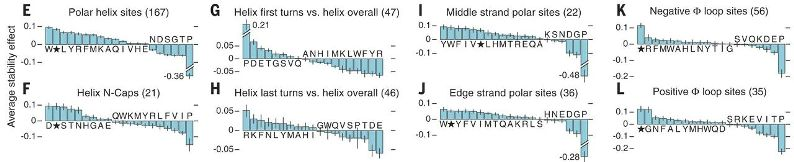
\includegraphics{stabilityTable}
\caption%[]
{
Efecto sobre la estabilidad de mutaciones en diferentes contextos estructurales. 
Los valores negativos, como los de la prolina en general, son desestabilizadores. 
Adaptada de \citet{Rocklin2017}. Copyright (2017) Science.
}
\label{fig:miniprotstab} %https://www.ncbi.nlm.nih.gov/pmc/articles/PMC5568797/
\end{center}
\end{figure}

\begin{figure}
\begin{center} 
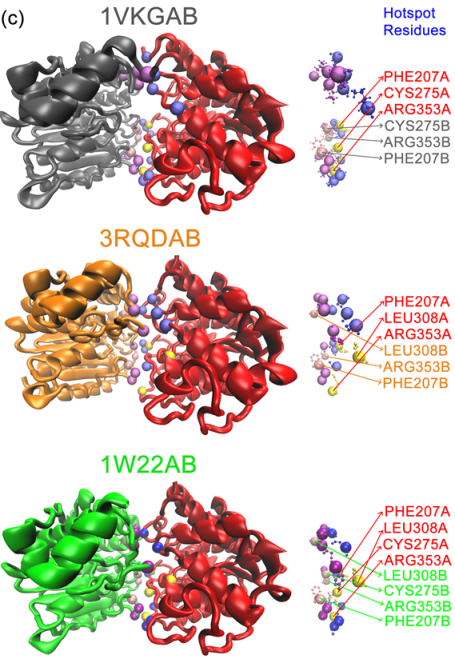
\includegraphics{ppi_interface}
\caption%[]
{
Grafo de la interfaz entre una histona-deacetilasa (en rojo) y tres parejas distintas.
Figura tomada de \citet{Cukuroglu2014} y reproducida con permiso de los autores.
}
\label{fig:ppi_interface}
\end{center}
\end{figure}

%\begin{figure}
%\begin{center} 
%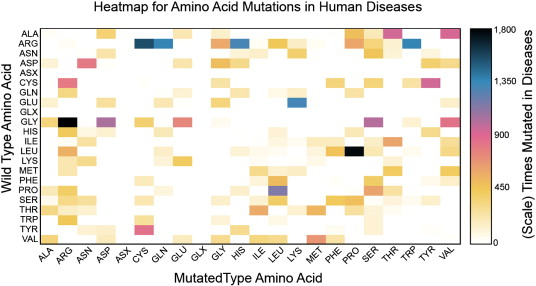
\includegraphics{human_mutations_heatmap}
%\caption%[]
%{
%Frecuencias de sustituci\'{o}n de amino\'{a}cidos en enfermedades humanas.
%Figura tomada de \citet{Peterson2013} y reproducida con permiso.}
%\label{fig:human_mutations_heatmap} %https://www.ncbi.nlm.nih.gov/pmc/articles/PMC3807015/
%\end{center}
%\end{figure}

Como se muestra en la figura \ref{fig:SNPpredictors}, hay una gran variedad de m\'{e}todos para la inferencia del fenotipo
molecular de mutaciones puntuales en prote\'{i}nas, y solamente algunos usan informaci\'{o}n estructural.
Probablemente el m\'{a}s universal de todos sea SIFT \citep{Kumar2009}, que usa como evidencia la
historia evolutiva de cada familia de prote\'{i}nas, que integra entre otras cosas determinantes estructurales
siempre y cuando haya suficientes secuencias hom\'{o}logas conocidas \citep{Saunders2002}. 
Sin embargo, como ocurre a menudo en biolog\'{i}a computacional, no es sencillo averiguar a partir de un
an\'{a}lisis de la literatura qu\'{e} m\'{e}todos son mejores. Hay que probarlos y escoger, y entre los
disponibles haya cada vez m\'{a}s alternativas que hacen un uso expl\'{i}cito de informaci\'{o}n
estructural, en concreto del contexto del residuo sustituido, como PolyPhen-2 \citep{Adzhubei2010},
SusPect \citep{Yates2014} o mCSM \citep{Pires2014}.

\begin{figure}
\begin{center} 
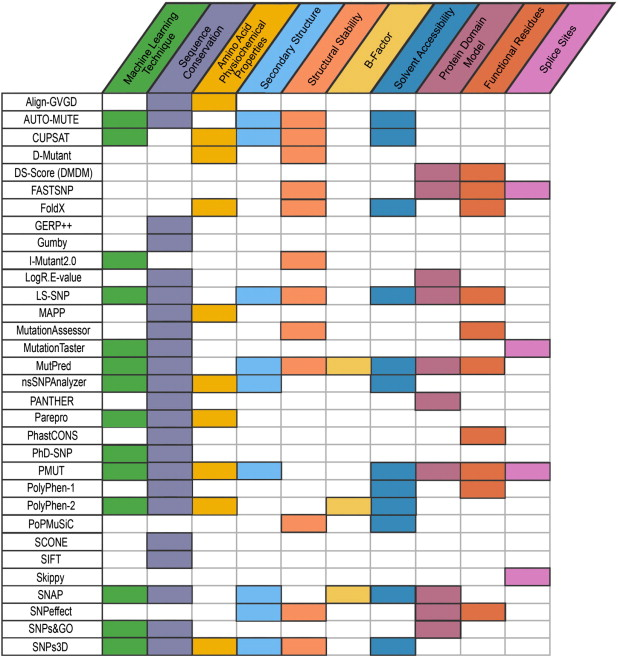
\includegraphics{SNPpredictors}
\caption%[]
{
Clasificaci\'{o}n de m\'{e}todos de inferencia de fenotipos de mutaciones no sin\'{o}nimas en base a los tipos de datos que emplean.
Figura tomada de \citet{Peterson2013} y reproducida con permiso.
}
\label{fig:SNPpredictors}
\end{center}
\end{figure}

\begin{figure}
\begin{center} 
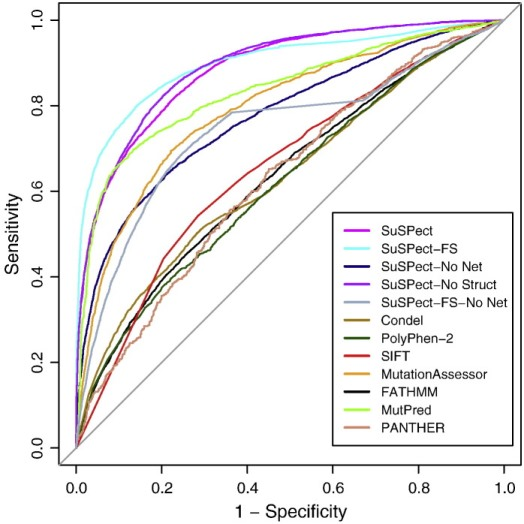
\includegraphics{SNP_performance}
\caption%[]
{
Comparaci\'{o}n del rendimiento de SusPect prediciendo mutaciones humanas delet\'{e}reas frente a otros predictores.
Figura tomada de \citep{Yates2014} y reproducida con permiso.
}
\label{fig:SNP_performance} %https://www.ncbi.nlm.nih.gov/pmc/articles/PMC4087249/
\end{center}
\end{figure}

Para explorar la predicci\'{o}n de fenotipos de mutaciones no sin\'{o}nimas planteo este ejercicio:
\begin{itemize}

\item Visita una base de datos de mutantes, como \htmladdnormallink{OMIM}{http://www.omim.org}, y elige una prote\'{i}na P (ejemplo: OPCML).

\item Obt\'{e}n la secuencia silvestre de amino\'{a}cidos S y al menos otra M con una mutaci\'{o}n delet\'{e}rea.

\item Construye un modelo comparativo de M y S.

\item Haz predicciones de fenotipo para S y M con ayuda, por ejemplo, de: \htmladdnormallink{SIFT}{http://sift.jcvi.org/}, 
\htmladdnormallink{PolyPhen-2}{http://genetics.bwh.harvard.edu/pph2/} y \htmladdnormallink{SusPect}{http://www.sbg.bio.ic.ac.uk/~suspect}.

\item Compara las predicciones obtenidas e interpr\'{e}talas a la luz de las estructuras modeladas. 
Qu\'{e} limitaciones del modelado comparativo afloran?

\end{itemize}
